% 包含图片的文件编译比较慢, 可以注释掉图片, 需要的时候再去掉注释

% TODO:
% 习题 1.1
% 习题 1.2 中心应该是 $(-1,0,\cdots,0)$
% 引理 2.3 中的记号太复杂了, 有空的话可以用序列的语言重写
% 习题 2.4
% 习题 3.2 需要求出 $\mathbb{F}_2\mathbb{P}^2$ 中处于一般位置的点组(给定一个点的情况下)的个数

\documentclass{ctexart}
\usepackage{lecturenote}
\title{第5章笔记和习题}

\begin{document}
\maketitle
在这章中, 不加说明的话, $\mathbb{A}$ 一律为与域 $K$ 上的 $n$ 维线性空间 $V$ 相伴的仿射空间, $\mathbb{E}$ 一律为与域 $K$ 上的 $n$ 维 Euclid 空间 $V$ 相伴的仿射空间.
\section{二次函数(对应第 1 节)}
\subsection{二次函数}
设 $\phi:\mathbb{A}\times\mathbb{A}\to K$ 是双仿射的, 给定 $\mathbb{A}$ 的一个坐标系 $\{\dot{o},\boldsymbol{e}_1,\boldsymbol{e}_2,\cdots,\boldsymbol{e}_n\}$, $\dot{p}$ 的坐标为 $X=[x_1,x_2,\cdots,x_n]$, $\dot{q}$ 的坐标为 $Y=[y_1,y_2,\cdots,y_n]$. 有
\begin{align*}
    \phi(\dot{p},\dot{q}) & =\phi(\dot{o},\dot{q})+\sum\limits_{i=1}^n\xi_i(\dot{q})x_i \\
    & =\phi(\dot{o},\dot{o})+\sum\limits_{i=1}^nb_iy_i+\sum\limits_{i=1}^n\left(\sum\limits_{j=1}^nc_{ij}y_j+a_i\right)x_i \\
    & =\phi(\dot{o},\dot{o})+{}^tAX+{}^tBY+{}^tXCY,
\end{align*}

其中 $A=[a_1,a_2,\cdots,a_n],B=[b_1,b_2,\cdots,b_n],C=(c_{ij})$. 如果 $\phi$ 是对称的, 则
\[\phi(\dot{p},\dot{q})=\phi(\dot{o},\dot{o})+{}^tAX+{}^tAY+{}^tXCY,\]

其中 $C$ 是对称的.

反之, 对于具有形式
\[\phi(\dot{p},\dot{q})=\phi_0+{}^tAX+{}^tBY+{}^tXCY,\quad A,B\in K^n,C\in M_n(K),\phi_0\in K\]
的函数 $\phi$, 固定 $\dot{q}$(等价于固定 $Y$), 则
\begin{align*}
    \phi(\dot{p},\dot{q}) & =(\phi_0+{}^tBY)+{}^tAX+{}^tXCY \\
    & =(\phi_0+{}^tBY)+{}^tAX+{}^tY{}^tCX \\
    & =(\phi_0+{}^tBY)+({}^tA+{}^tY{}^tC)X \\
\end{align*}
是 $\dot{p}$ 的仿射函数. 同理, 固定 $\dot{p}$, 则 $\phi$ 是 $\dot{q}$ 的仿射函数. $\therefore\mathbb{A}$ 上的双仿射函数与 $K\times K^n\times K^n\times M_n(K)$ 间可以建立双射. 下面将双仿射函数与
\[\phi(\dot{p},\dot{q})=\phi_0+{}^tAX+{}^tBY+{}^tXCY,\quad A,B\in K^n,C\in M_n(K),\phi_0\in K\]
等同起来.

我们希望能找到不依赖于坐标系的选取的性质. 考虑对称的双仿射函数
\begin{equation}\label{eq1.1}
    \phi(\dot{p},\dot{q})=\phi_0+{}^tAX+{}^tAY+{}^tXCY,\quad A\in K^n,C\in M_n(K),{}^tC=C,\phi_0\in K.
\end{equation}

设 $\{\dot{o}',\boldsymbol{e}_1',\boldsymbol{e}_2',\cdots,\boldsymbol{e}_n'\}$ 是 $\mathbb{A}$ 的另一个坐标系, 且
\[(\boldsymbol{e}_1',\boldsymbol{e}_2',\cdots,\boldsymbol{e}_n')=(\boldsymbol{e}_1,\boldsymbol{e}_2,\cdots,\boldsymbol{e}_n)F,\quad\overrightarrow{o'o}=(\boldsymbol{e}_1',\boldsymbol{e}_2',\cdots,\boldsymbol{e}_n')B,\quad B\in K^n,\]

则
\begin{equation}\label{eq1.2}
    \overrightarrow{o'p}=\overrightarrow{o'o}+\overrightarrow{op}=(\boldsymbol{e}_1',\boldsymbol{e}_2',\cdots,\boldsymbol{e}_n')(B+X).
\end{equation}

设 $\dot{p}$ 在 $\{\dot{o}',\boldsymbol{e}_1',\boldsymbol{e}_2',\cdots,\boldsymbol{e}_n'\}$ 下的坐标为 $X'$, 则
\begin{equation}\label{eq1.3}
    \overrightarrow{o'p}=(\boldsymbol{e}_1',\boldsymbol{e}_2',\cdots,\boldsymbol{e}_n')X'=(\boldsymbol{e}_1,\boldsymbol{e}_2,\cdots,\boldsymbol{e}_n)FX'.
\end{equation}

比较 (\ref{eq1.2}), (\ref{eq1.3}) 两式, 得
\[FX'=B+X\Rightarrow X=FX'-B.\]

同理得 $Y=FY'-B$. 代入 (\ref{eq1.1}) 式得
\begin{align*}
    \phi(\dot{p},\dot{q}) & =\phi_0+{}^tA(FX'-B)+{}^tA(FY'-B)+{}^t(FX'-B)C(FY'-B) \\
    & =\phi_0+{}^tAFX'-{}^tAB+{}^tAFY'-{}^tAB+({}^tX'{}^tF-{}^tB)C(FY'-B) \\
    & =\phi_0+{}^tBCB-2{}^tAB+{}^tAFX'+{}^tAFY'+{}^tX'{}^tFCFY'-{}^tX'{}^tFCB-{}^tBCFY' \\
    & =(\phi_0+{}^tBCB-2{}^tAB)+{}^tAFX'+({}^tAF-{}^tBCF)Y'+{}^tX'{}^tFCFY'-{}^tB{}^tCFX' \\
    & =(\phi_0+{}^tBCB-2{}^tAB)+({}^tAF-{}^tB{}^tCF)X'+({}^tAF-{}^tBCF)Y'+{}^tX'{}^tFCFY',
\end{align*}

考察 $\phi(\dot{p},\dot{q})$ 的二次部分, 其在 $\{\dot{o}',\boldsymbol{e}_1',\boldsymbol{e}_2',\cdots,\boldsymbol{e}_n'\}$ 下的系数矩阵为 ${}^tFCF$. $\because F\in\operatorname{GL}_n$, $\therefore\operatorname{rank}C=\operatorname{rank}{}^tFCF$, 即 $\phi(\dot{p},\dot{q})$ 的二次部分的系数矩阵的秩与坐标的选取无关. 记 $\operatorname{rank}\phi=\operatorname{rank}C$.

跟前一章一样, 将线性空间与仿射空间中的函数的概念做比较, 如表 \ref{tb1}.
\begin{table}\caption{线性空间与仿射空间的概念}\label{tb1}
    \begin{center}
        \begin{tabular}{c|c}
            线性空间 & 仿射空间 \\
            \hline
            线性函数 & 仿射函数 \\
            双线性型 & 双仿射函数 \\
            二次型 & 二次函数 \\
        \end{tabular}
    \end{center}
\end{table}
\subsection{二次函数的中心}
从一个简单的例子引出中心的定义.
\begin{example}
    考察圆 $(x-a)^2+(y-b)^2=r^2$, 对应的二次函数为 $Q([x,y])=(x-a)^2+(y-b)^2-r^2$, $Q$ 的二次部分为一个二次型 $q([x,y])=x^2+y^2$, 则有
    \begin{equation}\label{eq1.4}
        Q([x+a,y+b])=x^2+y^2-r^2=q([x,y])+Q([a,b]).
    \end{equation}
    
    上式完全刻画了 $[a,b]$ 作为圆的中心这一性质, 即 $[a,b]$ 是圆的中心当且仅当上式成立. 事实上, 设 $[c,d]$ 满足 $\forall x,y\in\mathbb{R}$,
    \[Q([x+c,y+d])=q([x,y])+Q([c,d]),\]

    上式两边减式 (\ref{eq1.4}), 得
    \begin{align*}
        & Q([x+c,y+d])-Q([x+a,y+b])=Q([c,d])-Q([a,b]) \\
        \Rightarrow &\ ((x+c-a)^2+(y+d-b)^2-r^2)-(x^2+y^2-r^2)=(c-a)^2+(d-b)^2-r^2-r^2 \\
        \Rightarrow &\ (x+c-a)^2+(y+d-b)^2-x^2-y^2=(c-a)^2+(d-b)^2 \\
        \Rightarrow &\ x^2+(c-a)^2+2x(c-a)+y^2+(d-b)^2+2y(d-b)-x^2-y^2=(c-a)^2+(d-b)^2 \\
        \Rightarrow &\ 2x(c-a)+2y(d-b)=0.
    \end{align*}

    $\because$ 上式对 $\forall x,y\in\mathbb{R}$ 成立, $\therefore c-a=d-b=0$.
\end{example}
一般的二次函数 $Q(\dot{p})$ 有类似于 (\ref{eq1.1}) 式的分解式:
\[Q(\dot{o}+\boldsymbol{x})=Q(\dot{o})+2l(\boldsymbol{x})+q(\boldsymbol{x}),\]

其中 $q(\boldsymbol{x})$ 为二次型, $l(\boldsymbol{x})$ 为线性映射. 定义
\begin{definition}\label{d1.1}
    如果对 $\forall\boldsymbol{u}\in V,Q(\dot{p}+\boldsymbol{u})=Q(\dot{p})+q(\boldsymbol{u})$, 则称 $\dot{p}$ 为 $Q$ 的\textbf{中心}.
\end{definition}
二次函数的中心不一定唯一, 也可以没有中心, 比如
\begin{example}
    $\mathbb{A}=\mathbb{R}^3$ 中的柱面 $x^2+y^2=r^2$ 对应的二次函数 $Q([x,y,z])=x^2+y^2-r^2$, 中心具有 $[0,0,c]\ (c\in\mathbb{R})$ 的形式.
\end{example}
在上面的例子中, 有 $\forall c\in\mathbb{R},Q([0,0,c])=Q([0,0,0])=-r^2$. 一般地, 有
\begin{theorem}\label{t1.1}
    设 $\dot{p},\dot{s}\in C(Q)$, 则 $Q(\dot{p})=Q(\dot{s})$.
\end{theorem}
\begin{proof}
    有
    \[Q(\dot{s})=Q(\dot{p}+\overrightarrow{ps})=Q(\dot{p})+q(\overrightarrow{ps}),\quad Q(\dot{p})=Q(\dot{s}+\overrightarrow{sp})=Q(\dot{s})+q(\overrightarrow{sp}),\]

    两式相减, 得
    \[Q(\dot{s})-Q(\dot{p})=Q(\dot{p})-Q(\dot{s})+q(\overrightarrow{ps})-q(-\overrightarrow{ps}).\]

    $\because q(-\overrightarrow{ps})=q(\overrightarrow{ps})$, $\therefore$
    \[Q(\dot{s})-Q(\dot{p})=Q(\dot{p})-Q(\dot{s})\Rightarrow Q(\dot{s})=Q(\dot{p}).\qedhere\]
\end{proof}
设 $f(\boldsymbol{x},\boldsymbol{x})$ 是与 $Q$ 配极的双线性型, $C(Q)$ 为 $Q$ 的中心的全体, 则
\begin{theorem}\label{t1.2}
    $\dot{p}=\dot{o}+\boldsymbol{x}\in C(Q)$ 当且仅当 $\forall\boldsymbol{y},f(\boldsymbol{x},\boldsymbol{y})+l(\boldsymbol{y})=0$.
\end{theorem}
\begin{proof}
    对 $\boldsymbol{y}\in V$, 有
    \begin{align*}
        Q(\dot{p}+\boldsymbol{y}) & =Q(\dot{o}+\boldsymbol{x}+\boldsymbol{y}) \\
        & =q(\boldsymbol{x}+\boldsymbol{y})+2l(\boldsymbol{x}+\boldsymbol{y})+Q(\dot{o}).
    \end{align*}

    $\because q(\boldsymbol{x})=f(\boldsymbol{x},\boldsymbol{x})$, 其中 $f$ 是对称的双线性型, $\therefore$
    \begin{align*}
        q(\boldsymbol{x}+\boldsymbol{y})+2l(\boldsymbol{x}+\boldsymbol{y})+Q(\dot{o}) & =q(\boldsymbol{x})+q(\boldsymbol{y})+2f(\boldsymbol{x},\boldsymbol{y})+2l(\boldsymbol{x})+2l(\boldsymbol{y})+Q(\dot{o}) \\
        & =Q(\dot{p})+q(\boldsymbol{y})+2f(\boldsymbol{x},\boldsymbol{y})+2l(\boldsymbol{y}).
    \end{align*}

    由定义 \ref{d1.1} 即得.
\end{proof}
设 $(\boldsymbol{e}_1,\boldsymbol{e}_2,\cdots,\boldsymbol{e}_n)$ 是 $V$ 的一个基, 则 $\forall\boldsymbol{y}\in V,\exists a_i\in K$ 使得 $\boldsymbol{y}=\sum\limits_{i=1}^na_i\boldsymbol{e}_i\Rightarrow f(\boldsymbol{x},\boldsymbol{y})+l(\boldsymbol{y})=\sum\limits_{i=1}^na_i(f(\boldsymbol{x},\boldsymbol{e}_i)+l(\boldsymbol{e}_i))$. $\therefore\forall\boldsymbol{y}\in V,f(\boldsymbol{x},\boldsymbol{y})+l(\boldsymbol{y})=0$ 等价于
\[f(\boldsymbol{x},\boldsymbol{e}_i)+l(\boldsymbol{e}_i)=0,\quad i=1,2,\cdots,n.\]

这是一个关于 $\boldsymbol{x}$ 的线性方程组, 这个方程组有没有解决定了 $C(Q)$ 是否非空.

设 $\phi_i=l(\boldsymbol{e}_i)$, $f$ 在基 $(\boldsymbol{e}_i)$ 下的矩阵为 $F=(f_{ij})$, $\boldsymbol{x}=(\boldsymbol{e}_1,\boldsymbol{e}_2,\cdots,\boldsymbol{e}_n)[x_1,x_2,\cdots,x_n]$, 可以把方程组重写为
\begin{equation}\label{eq1.5}
    \sum\limits_{j=1}^nf_{ij}x_j+\phi_i=0,\quad i=1,2,\cdots,n.
\end{equation}

方程组 \ref{eq1.5} 对应的齐次方程组为
\[\sum\limits_{j=1}^nf_{ij}x_j=0,\quad i=1,2,\cdots,n,\]

解空间为
\[\{X\in K^n|FX=0\}=\{X\in K^n|\forall Y\in K^n,{}^tYFX=0\}=\ker f.\]

其中 $\ker f$ 的定义见书上 P29\footnote{那里只定义了左核, 但定义的方式类似}. 由第 4 章笔记的定理 1.8 得方程组 \ref{eq1.5} 的解空间为以 $\ker f$ 为方向平面的仿射平面.
\subsection{二次函数的标准型}
将书上的定理 2,3 拆成几个定理.
\begin{theorem}\label{t1.3}
    设 $Q$ 是 $\mathbb{A}$ 上的二次函数, 如果 $C(Q)\neq\varnothing$, 则 $\exists$ 坐标系 $\{\dot{o},\boldsymbol{e}_1,\boldsymbol{e}_2,\cdots,\boldsymbol{e}_n\}$ 使得 $\forall\boldsymbol{x}\in V$,
    \[Q(\dot{o}+\boldsymbol{x})=\alpha_1x^2_1+\alpha_2x^2_2+\cdots+\alpha_rx^2_r+\phi_0,\]

    其中 $\boldsymbol{x}=(\boldsymbol{e}_1,\boldsymbol{e}_2,\cdots,\boldsymbol{e}_n)[x_1,x_2,\cdots,x_n],r=\operatorname{rank}Q$.
\end{theorem}
\begin{proof}
    取 $\dot{o}\in C(Q)$, 则
    \[Q(\dot{o}+\boldsymbol{v})=Q(\dot{o})+q(\boldsymbol{v}).\]

    由定理 \ref{t1.1}, 上式右边第一项与 $\dot{o}\in C(Q)$ 的选取无关, 为常数 $\phi_0$.

    由书上第 1 章第 4 节定理 4 的推论 1, $\exists V$ 的一个基 $\boldsymbol{e}_1,\boldsymbol{e}_2,\cdots,\boldsymbol{e}_n$ 使得 $q$ 在基 $\boldsymbol{e}_1,\boldsymbol{e}_2,\cdots,\boldsymbol{e}_n$ 下取规范形式, 即 $\forall\boldsymbol{x}\in V$,
    \[q(\boldsymbol{x})=\alpha_1x^2_1+\alpha_2x^2_2+\cdots+\alpha_rx^2_r.\qedhere\]
\end{proof}
\begin{lemma}\label{l1.1}
    有中心和没有中心的二次函数不会仿射等价.
\end{lemma}
\begin{proof}
    假设二次函数 $Q$ 没有中心且 $Q$ 与有中心的二次函数仿射等价, 由定理 \ref{t1.3} 得 $Q$ 在某个坐标系 $\{\dot{o},\boldsymbol{e}_1,\boldsymbol{e}_2,\cdots,\boldsymbol{e}_n\}$ 下有形式
    \[Q(\dot{o}+\boldsymbol{x})=\alpha_1x^2_1+\alpha_2x^2_2+\cdots+\alpha_rx^2_r+\phi_0=f(\boldsymbol{x},\boldsymbol{x})+\phi_0.\]

    $\because\boldsymbol{x}=\boldsymbol{0}$ 满足 $\forall\boldsymbol{y}=(\boldsymbol{e}_1,\boldsymbol{e}_2,\cdots,\boldsymbol{e}_n)Y\in V,f(\boldsymbol{x},\boldsymbol{y})+0Y=f(\boldsymbol{0},\boldsymbol{y})=0$, 由定理 \ref{t1.2} 得 $\dot{o}\in C(Q)$, 与 $C(Q)=\varnothing$ 矛盾.
\end{proof}
\begin{theorem}
    设 $Q$ 是 $\mathbb{A}$ 上的二次函数, 如果 $C(Q)=\varnothing$, 则 $\exists$ 坐标系 $\{\dot{o},\boldsymbol{e}_1,\boldsymbol{e}_2,\cdots,\boldsymbol{e}_n\}$ 使得 $\forall\boldsymbol{x}\in V$,
    \[Q(\dot{o}+\boldsymbol{x})=\alpha_1x^2_1+\alpha_2x^2_2+\cdots+\alpha_rx^2_r+2x_{r+1},\]

    其中 $\boldsymbol{x}=(\boldsymbol{e}_1,\boldsymbol{e}_2,\cdots,\boldsymbol{e}_n)[x_1,x_2,\cdots,x_n],r=\operatorname{rank}Q$.
\end{theorem}
\begin{proof}
    设 $f$ 是 $Q$ 的二次部分 $q$ 对应的双线性型. $\because C(Q)=\varnothing,\therefore$ 方程组 (\ref{eq1.5})\footnote{在方程组中出现的记号的含义与方程组前面的定义一致.} 没有解, $\therefore r=\operatorname{rank}f<n$.

    由书上第 1 章第 4 节定理 4 的推论 1, $\exists V$ 的一个基 $\boldsymbol{e}_1,\boldsymbol{e}_2,\cdots,\boldsymbol{e}_n$ 使得 $q$ 在基 $\boldsymbol{e}_1,\boldsymbol{e}_2,\cdots,\boldsymbol{e}_n$ 下取规范形式, 即 $\forall\boldsymbol{x}\in V$,
    \[q(\boldsymbol{x})=\alpha_1x^2_1+\alpha_2x^2_2+\cdots+\alpha_rx^2_r.\]

    $\therefore$ 在坐标系 $\{\dot{o},\boldsymbol{e}_1,\boldsymbol{e}_2,\cdots,\boldsymbol{e}_n\}$ 下有
    \[Q(\dot{o}+\boldsymbol{x})=\alpha_1x^2_1+\cdots+\alpha_rx^2_r+2(\beta_1x_1+\cdots+\beta_nx_n)+\phi_0.\]

    按书上 P150 的式 (3) 来刻画仿射变换. 作仿射变换
    \[g:x_i'=\begin{cases}
        x_i+\dfrac{\beta_i}{\alpha_i}, & 1\leq i\leq r, \\
        x_i, & r+1\leq i\leq n, \\
    \end{cases}\]

    设 $g(\dot{o})=\dot{o}',Dg\boldsymbol{x}=\boldsymbol{x}'$, 则
    \[Q(\dot{o}'+\boldsymbol{x}')=\alpha_1x'^2_1+\cdots+\alpha_rx'^2_r+2(\beta_{r+1}'x'_{r+1}+\cdots+\beta_n'x'_n)+\phi_0'.\]

    由引理 \ref{l1.1} 的证明得 $\beta_{r+1}',\beta_{r+2}',\cdots,\beta_n'$ 不全为 $0$. 设 $\beta_{r+1}'=\cdots=\beta_{r+k-1}'=0,\beta'_{r+k}\neq0$, 作仿射变换
    \[h:x''_i=\begin{cases}
        \beta'_{r+k}x'_{r+k}+\beta'_{r+k+1}x'_{r+k+1}+\cdots+\beta'_nx'_n+\dfrac{\phi_0}{2}, & i=r+1, \\
        x'_{i-1}, & r+1\leq i\leq r+k, \\
        x'_i, & \text{其他情况}, \\
    \end{cases},\]

    设 $h(\dot{o}')=\dot{o}'',Dh\boldsymbol{x}'=\boldsymbol{x}''$, 则
    \[Q(\dot{o}''+\boldsymbol{x}'')=\alpha_1x''^2_1+\cdots+\alpha_rx''^2_r+2x''_{r+1}.\]
\end{proof}
\begin{theorem}
    设 $Q$ 是 $\mathbb{E}$ 上的二次函数, 如果 $C(Q)\neq\varnothing$, 则 $\exists$ 直角坐标系 $\{\dot{o},\boldsymbol{e}_1,\boldsymbol{e}_2,\cdots,\boldsymbol{e}_n\}$ 使得 $\forall\boldsymbol{x}\in V$,
    \[Q(\dot{o}+\boldsymbol{x})=\lambda_1x^2_1+\lambda_2x^2_2+\cdots+\lambda_rx^2_r+\phi_0,\]

    其中 $\boldsymbol{x}=(\boldsymbol{e}_1,\boldsymbol{e}_2,\cdots,\boldsymbol{e}_n)[x_1,x_2,\cdots,x_n],r=\operatorname{rank}Q$, $\lambda_i$ 在不计重数的意义下是唯一的.
\end{theorem}
\begin{proof}
    取 $\dot{o}\in C(Q)$, 则
    \[Q(\dot{o}+\boldsymbol{v})=Q(\dot{o})+q(\boldsymbol{v}).\]

    由定理 \ref{t1.1}, 上式右边第一项与 $\dot{o}\in C(Q)$ 的选取无关, 为常数 $\phi_0$.

    由书上第 3 章第 3 节的定理 7, $\exists V$ 的一个标准正交基 $\boldsymbol{e}_1,\boldsymbol{e}_2,\cdots,\boldsymbol{e}_n$ 使得 $q$ 在基 $\boldsymbol{e}_1,\boldsymbol{e}_2,\cdots,\boldsymbol{e}_n$ 下取规范形式, 即 $\forall\boldsymbol{x}\in V$,
    \[q(\boldsymbol{x})=\lambda_1x^2_1+\lambda_2x^2_2+\cdots+\lambda_rx^2_r.\]

    $\because\lambda_i$ 是 $q$ 的特征值, $\therefore\lambda_i$ 在不计重数的意义下是唯一的.
\end{proof}
\begin{theorem}
    设 $Q$ 是 $\mathbb{E}$ 上的二次函数, 如果 $C(Q)=\varnothing$, 则 $\exists$ 直角坐标系 $\{\dot{o},\boldsymbol{e}_1,\boldsymbol{e}_2,\cdots,\boldsymbol{e}_n\}$ 使得 $\forall\boldsymbol{x}\in V$,
    \[Q(\dot{o}+\boldsymbol{x})=\lambda_1x^2_1+\lambda_2x^2_2+\cdots+\lambda_rx^2_r+2\mu x_{r+1},\]

    其中 $\boldsymbol{x}=(\boldsymbol{e}_1,\boldsymbol{e}_2,\cdots,\boldsymbol{e}_n)[x_1,x_2,\cdots,x_n],r=\operatorname{rank}Q,\lambda_i,\mu$ 在不计重数的意义下是唯一的.
\end{theorem}
\begin{proof}
    设 $f$ 是 $Q$ 的二次部分 $q$ 对应的双线性型. $\because C(Q)=\varnothing,\therefore$ 方程组 (\ref{eq1.5}) 没有解, $\therefore r=\operatorname{rank}f<n$.

    由书上第 3 章第 3 节的定理 7, $\exists V$ 的一个标准正交基 $\boldsymbol{e}_1,\boldsymbol{e}_2,\cdots,\boldsymbol{e}_n$ 使得 $q$ 在基 $\boldsymbol{e}_1,\boldsymbol{e}_2,\cdots,\boldsymbol{e}_n$ 下取规范形式, 即 $\forall\boldsymbol{x}\in V$,
    \[q(\boldsymbol{x})=\lambda_1x^2_1+\lambda_2x^2_2+\cdots+\lambda_rx^2_r.\]

    $\therefore$ 在坐标系 $\{\dot{o},\boldsymbol{e}_1,\boldsymbol{e}_2,\cdots,\boldsymbol{e}_n\}$ 下有
    \[Q(\dot{o}+\boldsymbol{x})=\lambda_1x^2_1+\cdots+\lambda_rx^2_r+2(\beta_1x_1+\cdots+\beta_nx_n)+\phi_0.\]

    $\because\lambda_i$ 是 $q$ 的特征值, $\therefore\lambda_i$ 在不计重数的意义下是唯一的.

    作平移
    \[g:x_i'=\begin{cases}
        x_i+\dfrac{\beta_i}{\lambda_i}, & 1\leq i\leq r, \\
        x_i, & r+1\leq i\leq n, \\
    \end{cases}\]

    设 $g(\dot{o})=\dot{o}',Dg\boldsymbol{x}=\boldsymbol{x}'$, 则
    \[Q(\dot{o}'+\boldsymbol{x}')=\lambda_1x'^2_1+\cdots+\lambda_rx'^2_r+2(\beta_{r+1}'x'_{r+1}+\cdots+\beta_n'x'_n)+\phi_0'.\]

    $\because f$ 在基 $(\boldsymbol{e}_i)$ 下的矩阵为
    \[\begin{pmatrix}
        \lambda_1 \\
        & \ddots \\
        && \lambda_r \\
        &&& 0 \\
        &&&& \ddots \\
        &&&&& 0 \\
    \end{pmatrix},\]

    $\therefore\ker f=\left<\boldsymbol{e}_{r+1},\boldsymbol{e}_{r+2},\cdots,\boldsymbol{e}_n\right>$.

    $\therefore$
    \[Q(\dot{o}'+\boldsymbol{x}')=q(\boldsymbol{u})+2l(\boldsymbol{v})+\phi_0',\]

    其中 $\boldsymbol{u}\in(\ker f)^\perp,\boldsymbol{v}\in\ker f,l\in(\ker f)^*$. $\because\ker f$ 是 Euclid 向量空间, 由书上第 3 章第 1 节的定理 7 得 $(\ker f)^*\simeq\ker f$.
    
    设 $e^{r+1},e^{r+2},\cdots,e^n$ 是 $(\ker f)^*$ 中与 $\boldsymbol{e}_{r+1},\boldsymbol{e}_{r+2},\cdots,\boldsymbol{e}_n$ 对偶的基, 则 $l$ 在基 $e^{r+1},e^{r+2},\cdots,e^n$ 下的坐标为 $[\beta'_{r+1},\beta'_{r+2},\cdots,\beta'_n]$. $\because(\ker f)^*\simeq\ker f$, $\therefore\exists\boldsymbol{l}\in\ker f,\boldsymbol{l}$ 在基 $\boldsymbol{e}_{r+1},\boldsymbol{e}_{r+2},\cdots,\boldsymbol{e}_n$ 下的坐标为 $[\beta'_{r+1},\beta'_{r+2},\cdots,\beta'_n]$.
    
    令 $\mu=\|\boldsymbol{l}\|=\sqrt{\beta'^2_{r+1}+\beta'^2_{r+2}+\cdots+\beta'^2_n}$, 则 $\mu$ 在 $\ker f$ 的正交算子作用下不变.

    作变换
    \[h:x''_j=\begin{cases}
        x'_j, & 1\leq j\leq r, \\
        \dfrac{1}{\mu}(\beta'_{r+1}x'_{r+1}+\beta'_{r+2}x'_{r+2}+\cdots+\beta'_nx'_n)+\dfrac{\phi_0}{2}, & j=r+1, \\
        \sum\limits_{i=r+1}^n\alpha_{ij}x'_i, & r+2\leq j\leq n, \\
    \end{cases},\]

    设 $h|_{\ker f}$ 在基 $\boldsymbol{e}_{r+1},\boldsymbol{e}_{r+2},\cdots,\boldsymbol{e}_n$ 下的矩阵为
    \[A=\begin{pmatrix}
        \dfrac{\beta'_{r+1}}{\mu} & \dfrac{\beta'_{r+2}}{\mu} & \cdots & \dfrac{\beta'_n}{\mu} \\
        \alpha_{r+2,r+1} & \alpha_{r+2,r+2} & \cdots & \alpha_{r+2,n} \\
        \vdots & \vdots & \ddots & \vdots \\
        \alpha_{n1} & \alpha_{n2} & \cdots & \alpha_{nn} \\
    \end{pmatrix}.\]

    $A_{(1)}$ 为单位矩阵, $\therefore A_{(1)}$ 可以扩充为 $K^n$ 的一个标准正交基 $A_{(1)},X_2,X_3,\cdots,X_n$. 令 $A_{(i)}=X_i\ (i=2,\cdots,n)$, 则 $A$ 为正交矩阵. $\therefore h\in\operatorname{Iso}(\mathbb{E})$.

    设 $h(\dot{o}')=\dot{o}'',Dh\boldsymbol{x}'=\boldsymbol{x}''$, 则
    \[Q(\dot{o}''+\boldsymbol{x}'')=\lambda_1x''^2_1+\cdots+\lambda_rx''^2_r+2\mu x''_{r+1}.\]

    设在直角坐标系 $\{\dot{o},\boldsymbol{e}_1',\boldsymbol{e}_2',\cdots,\boldsymbol{e}_n'\}$ 下有
    \[\boldsymbol{x}''=(\boldsymbol{e}_1',\boldsymbol{e}_2',\cdots,\boldsymbol{e}_n')[y''_1,y''_2,\cdots,y''_n],\quad Q(\dot{o}''+\boldsymbol{x}'')=\lambda_1y''^2_1+\cdots+\lambda_ry''^2_r+2\mu' y''_{r+1},\]

    则 $f$ 在基 $(\boldsymbol{e}_i)$ 和基 $(\boldsymbol{e}_i')$ 下的矩阵都为
    \[\begin{pmatrix}
        \Lambda & 0 \\
        0 & 0 \\
    \end{pmatrix}=\begin{pmatrix}
        \lambda_1 \\
        & \ddots \\
        && \lambda_r \\
        &&& 0 \\
        &&&& \ddots \\
        &&&&& 0 \\
    \end{pmatrix}.\]
    
    设 $(\boldsymbol{e}_1',\boldsymbol{e}_2',\cdots,\boldsymbol{e}_n')=(\boldsymbol{e}_1,\boldsymbol{e}_2,\cdots,\boldsymbol{e}_n)B$, 其中 $B$ 是正交矩阵, 则有
    \[\begin{pmatrix}
        \Lambda & 0 \\
        0 & 0 \\
    \end{pmatrix}={}^tB\begin{pmatrix}
        \Lambda & 0 \\
        0 & 0 \\
    \end{pmatrix}B=B^{-1}\begin{pmatrix}
        \Lambda & 0 \\
        0 & 0 \\
    \end{pmatrix}B.\]

    设 $B=\dbinom{B_1\quad B_2}{B_3\quad B_4}$, 其中 $B_1\in M_r(K),B_4\in M_{n-r}(K)$, 则
    \[\begin{pmatrix}
        B_1 & B_2 \\
        B_3 & B_4 \\
    \end{pmatrix}\begin{pmatrix}
        \Lambda & 0 \\
        0 & 0 \\
    \end{pmatrix}=\begin{pmatrix}
        \Lambda & 0 \\
        0 & 0 \\
    \end{pmatrix}\begin{pmatrix}
        B_1 & B_2 \\
        B_3 & B_4 \\
    \end{pmatrix}.\]

    $\therefore$
    \[\begin{pmatrix}
        \Lambda B_1 & 0 \\
        \Lambda B_3 & 0 \\
    \end{pmatrix}=\begin{pmatrix}
        \Lambda B_1 & \Lambda B_2 \\
        0 & 0 \\
    \end{pmatrix}, B_2=B_3=0.\]

    $\because B$ 是正交矩阵, $\therefore B_4$ 是正交矩阵. $\because\mu$ 在正交算子作用下不变, $\therefore\mu'=\mu$.
\end{proof}
\section{二次曲面(对应第 2 节)}
在这节中, 默认给出坐标系 $\{\dot{o},\boldsymbol{e}_1,\boldsymbol{e}_2,\cdots,\boldsymbol{e}_n\}$, 二次曲面和点都用坐标表示.
\subsection{一般概念}
$\mathbb{A}$ 上的二次曲面中与域 $K$ 有关, 比如
\begin{example}
    当 $K=\mathbb{R}$ 时, $\mathbb{A}$ 上的二次曲面 $x_1^2+x_2^2-1=0$ 是空集. 书上将空集称为``零''二次曲面.

    然而当 $K=\mathbb{R}$ 时, $\mathbb{A}$ 上的二次曲面 $x_1^2+x_2^2-1=0$ 非空.
\end{example}
当 $K$ 是代数闭域的时候, $\forall$ 二次函数 $Q$, $S_Q=\{\dot{p}|Q(\dot{p})=0\}$ 非空.

设 $K'\subset K$. 考察 $S_Q$ 中的点 $\dot{x}$. 设 $\dot{x}$ 在某个坐标系下的坐标为 $X$, 定义
\[S_Q(K')=\{\dot{x}|X\in K'^n\}.\]

在代数几何中会进一步研究 $S_Q(K')$. 下面只研究比较直观的 $K=\mathbb{R}$ 的情形.
\begin{example}
    (1) 设 $Q=\alpha_1x^2_1+\alpha_2x^2_2+\cdots+\alpha_rx^2_r\ (r\leq n)$, 则 $\boldsymbol{x}\in S_Q$ 当且仅当 $x_1=x_2=\cdots=x_r=0$. $\therefore$
    \[S_Q=\left\{\dot{o}+\boldsymbol{x}\Bigg|\boldsymbol{x}=\sum\limits_{i=r+1}^na_i\boldsymbol{e}_i,a_i\in\mathbb{R}\right\}.\]

    (2) 设 $Q=\alpha_1(x_1-s_1)^2+\alpha_2(x_2-s_2)^2+\cdots+\alpha_r(x_r-s_r)^2\ (r\leq n,s_i\in\mathbb{R})$, 则 $\boldsymbol{x}\in S_Q$ 当且仅当 $x_i=s_i\ (i=1,2,\cdots,r)$. $\therefore$
    \[S_Q=\left\{\dot{o}+\boldsymbol{x}\Bigg|\boldsymbol{x}=\sum\limits_{i=1}^rs_i\boldsymbol{e}_i+\sum\limits_{i=r+1}^na_i\boldsymbol{e}_i,a_i\in\mathbb{R}\right\}.\]
\end{example}
二重平面的图形比较简单, 但方程不是唯一确定的, 所以不是我们感兴趣的情形. 下面不加说明的话, 设 $S_Q$ 不是二重平面.

补充书上定理 1 用到的几个引理.
\begin{lemma}
    设 $S_Q$ 是二次曲面, $\dot{p},\dot{q}\in S_Q$, 设过 $\dot{p},\dot{q}$ 的直线为 $l_{\dot{p},\dot{q}}=\{\dot{p}+\lambda\overrightarrow{pq}|\lambda\in\mathbb{R}\}$. 若 $l_{\dot{p},\dot{q}}\not\subset S_Q$, 则 $l_{\dot{p},\dot{q}}\cap S_Q=\{\dot{p},\dot{q}\}$.
\end{lemma}
\begin{proof}
    $\forall\dot{r}\in l_{\dot{p},\dot{q}}$, 有 $\overrightarrow{or}=\overrightarrow{op}+\overrightarrow{pr}=\overrightarrow{op}+\lambda\overrightarrow{pq}$.

    设 $\overrightarrow{op}=\sum\limits_{i=1}^na_i\boldsymbol{e}_i,\overrightarrow{pq}=\sum\limits_{i=1}^nb_i\boldsymbol{e}_i$, 则
    \[\overrightarrow{or}=\sum\limits_{i=1}^na_i\boldsymbol{e}_i+\lambda\sum\limits_{i=1}^nb_i\boldsymbol{e}_i=\sum\limits_{i=1}^n(a_i+\lambda b_i)\boldsymbol{e}_i.\]

    $\therefore\dot{r}$ 的坐标为 $(a_1+\lambda b_1,a_2+\lambda b_2,\cdots,a_n+\lambda b_n)$.

    $\because Q(\dot{r})=0$ 是关于 $\lambda$ 的二次方程 $f(\lambda)=0$, $\therefore$ 若 $\exists\lambda_0$ 使得 $f(\lambda)\neq0$, 则方程 $f(\lambda)=0$ 至多有两个解. $\because f(0)=f(1)=0$, $\therefore\forall\lambda\in\mathbb{R}\backslash\{0,1\},f(\lambda)\neq0\Rightarrow\dot{p}+\lambda\overrightarrow{pq}\notin S_Q$.
\end{proof}
\begin{lemma}\label{l2.2}
    设 $K$ 是无限域, $f,g\in K[t_1,\cdots,t_n]$, 若 $\forall t_1,\cdots,t_n\in K,f(t_1,\cdots,t_n)=g(t_1,\cdots,t_n)$, 则 $f=g$.
\end{lemma}
\begin{proof}
    对变元的个数用数学归纳法. 由 [BAI] 第 6 章第 1 节定理 2 的推论得单变元的情形成立. 假设对 $f,g\in K[t_1,\cdots,t_{n-1}]$, 若 $\forall t_1,\cdots,t_{n-1}\in K,f(t_1,\cdots,t_{n-1})=g(t_1,\cdots,t_{n-1})$, 则 $f=g$.

    对 $f,g\in K[t_1,\cdots,t_{n-1}]$, 固定 $x_1,\cdots,x_{n-1}$, 设
    \[f_{x_1,\cdots,x_{n-1}}(t_n)=f(x_1,\cdots,x_{n-1},t_n)=\sum\limits_it_n^if_i(x_1,\cdots,x_{n-1}),\]
    \[g_{x_1,\cdots,x_{n-1}}(t_n)=g(x_1,\cdots,x_{n-1},t_n)=\sum\limits_it_n^ig_i(x_1,\cdots,x_{n-1}).\]

    $\because\forall t_n,f_{x_1,\cdots,x_{n-1}}(t_n)=g_{x_1,\cdots,x_{n-1}}(t_n)$, 由 [BAI] 第 6 章第 1 节定理 2 的推论得 $f_{x_1,\cdots,x_{n-1}}=g_{x_1,\cdots,x_{n-1}}$. $\therefore$
    \[f_i(x_1,x_2,\cdots,x_{n-1})=g_i(x_1,x_2,\cdots,x_{n-1}).\]

    $\because$ 上式对 $\forall x_1,\cdots,x_{n-1}$ 都成立, 由归纳假定, $f_i(t_1,\cdots,t_{n-1})=g_i(t_1,\cdots,t_{n-1})$. $\therefore$
    \[f(t_1,\cdots,t_n)=\sum\limits_it_n^if_i(t_1,\cdots,t_{n-1})=\sum\limits_it_n^ig_i(t_1,\cdots,t_{n-1})=g(t_1,\cdots,t_n).\qedhere\]
\end{proof}
书上定理 1 后半部分的证明需要用到分析的结论.
\begin{theorem}[书上定理 1 的后半部分]
    沿用书上定理 1 证明中的记号. 如果 $\Delta_1\geq0,\Delta_2\geq0$, 那么 $Q_1=Q_2$.
\end{theorem}
\begin{proof}
    $\because g_1,g_2,h_1,h_2$ 是连续函数, $\therefore\exists$ 球 $B_r(\boldsymbol{0})$ 使得 $\forall[x_1,\cdots,x_{n-1}]\in B_r(\boldsymbol{0}),g_i^2(x_1,\cdots,x_{n-1})-4h_i(x_1,\cdots,x_{n-1})\geq0,i=1,2$.

    $\therefore\forall[x_1,\cdots,x_{n-1}]\in B_r(\boldsymbol{0})$, 关于 $x_n$ 的方程 $Q_i(\dot{p}+\boldsymbol{x})=0,\ i=1,2$ 有两个实数解.

    $\because\forall\lambda_1,\lambda_2,\cdots,\lambda_{n-1}\in\mathbb{R},\exists t\in\mathbb{R}$ 使得 $[t\lambda_1,t\lambda_2,\cdots,t\lambda_{n-1}]\in B_r(\boldsymbol{0})$, $\therefore\forall\lambda_1,\lambda_2,\cdots,\lambda_{n-1}\in\mathbb{R},\exists$ 不相同的 $\dot{r}'=\dot{p}+\sum\limits_{i=1}^{n-1}t\lambda_i\boldsymbol{e}_i+x_n'\boldsymbol{e}_n,\dot{r}''=\dot{p}+\sum\limits_{i=1}^{n-1}t\lambda_i\boldsymbol{e}_i+x_n''\boldsymbol{e}_n$ 使得 $Q_1(\dot{r}')=Q_2(\dot{r}'')=0\Rightarrow\dot{r}',\dot{r}''\in S_{Q_1}$.

    $\because S_{Q_1}=S_{Q_2},\therefore\dot{r}',\dot{r}''\in S_{Q_2}$.

    考察二次方程
    \[f_i(x_n)=Q_i\left(\dot{p}+\sum\limits_{i=1}^{n-1}t\lambda_i\boldsymbol{e}_i+x_n\boldsymbol{e}_n\right)=0,\quad i=1,2.\]

    $\because\dot{r}',\dot{r}''\in S_{Q_i},\ i=1,2$, $\therefore f_i(x'_n)=f_i(x''_n)=0,\ i=1,2$.

    由 Vieta 公式,
    \begin{equation}\label{eq2.1}
        \begin{aligned}
            & g_1(t\lambda_1,t\lambda_2,\cdots,t\lambda_{n-1})=-x'_n-x''_n=g_2(t\lambda_1,t\lambda_2,\cdots,t\lambda_{n-1}), \\
            & h_1(t\lambda_1,t\lambda_2,\cdots,t\lambda_{n-1})=x'_nx''_n=h_2(t\lambda_1,t\lambda_2,\cdots,t\lambda_{n-1}).
        \end{aligned}
    \end{equation}

    式 \ref{eq2.1} 对 $\forall$ 充分小的 $t$ 都成立, $\therefore\exists$ 无穷多个 $t$ 满足式 \ref{eq2.1}. $\because$
    \[g_i(t\lambda_1,t\lambda_2,\cdots,t\lambda_{n-1}),\quad h_i(t\lambda_1,t\lambda_2,\cdots,t\lambda_{n-1}),\quad i=1,2\]
    是 $t$ 的多项式, $\therefore\forall t$, 式 \ref{eq2.1} 成立. 特别地,
    \begin{equation}\label{eq2.2}
        \begin{aligned}
            & g_1(\lambda_1,\lambda_2,\cdots,\lambda_{n-1})=-x'_n-x''_n=g_2(\lambda_1,\lambda_2,\cdots,\lambda_{n-1}), \\
            & h_1(\lambda_1,\lambda_2,\cdots,\lambda_{n-1})=x'_nx''_n=h_2(\lambda_1,\lambda_2,\cdots,\lambda_{n-1}).
        \end{aligned}
    \end{equation}

    上式对 $\forall\lambda_1,\lambda_2,\cdots,\lambda_{n-1}\in\mathbb{R}$ 成立. 由引理 \ref{l2.2} 得 $g_1=g_2,h_1=h_2$.
\end{proof}
书上 P197 的前几段可以总结为下面的定理:
\begin{theorem}
    $\dot{p}\in C(Q)$ 当且仅当 $\dot{p}$ 是 $S_q$ 的中心. 
\end{theorem}
\begin{proof}
    ($\Rightarrow$) $\because\dot{p}\in C(Q)$, $\therefore\forall\boldsymbol{x}\in V$,
    \[Q(\dot{p}+\boldsymbol{x})=q(\boldsymbol{x})+Q(\dot{p})=q(-\boldsymbol{x})+Q(\dot{p})=Q(\dot{p}-\boldsymbol{x}).\]

    ($\Leftarrow$) $\because\dot{p}$ 是 $S_q$ 的中心, $\therefore Q(\dot{p}+\boldsymbol{x})=0\Leftrightarrow Q(\dot{p}-\boldsymbol{x})=0$. $\therefore Q(\dot{p}+\boldsymbol{x})=0$ 和 $Q(\dot{p}-\boldsymbol{x})=0$ 定义了相同的曲面. 由书上的定理 1, $Q(\dot{p}+\boldsymbol{x})=\lambda Q(\dot{p}-\boldsymbol{x})\ (\lambda\in\mathbb{R})$. $\therefore\forall\boldsymbol{x}\in V$,
    \[q(\boldsymbol{x})+2l(\boldsymbol{x})+Q(\dot{p})=\lambda(q(\boldsymbol{-x})+2l(\boldsymbol{-x})+Q(\dot{p}))=\lambda(q(\boldsymbol{x})-2l(\boldsymbol{x})+Q(\dot{p})).\]

    $\therefore$
    \[(1-\lambda)(q(\boldsymbol{x})+Q(\dot{p}))+2(1+\lambda)l(\boldsymbol{x})=0.\]

    当 $\boldsymbol{x}=\boldsymbol{0}$ 时有 $q(\boldsymbol{x})=l(\boldsymbol{x})=0\Rightarrow(1-\lambda)Q(\dot{p})=0$. $\therefore$
    \begin{equation}\label{eq2.3}
        (1-\lambda)q(\boldsymbol{x})+2(1+\lambda)l(\boldsymbol{x})=0.
    \end{equation}

    在式 (\ref{eq2.3}) 中以 $-\boldsymbol{x}$ 代 $\boldsymbol{x}$, 得
    \[(1-\lambda)q(\boldsymbol{x})-2(1+\lambda)l(\boldsymbol{x})=(1-\lambda)q(-\boldsymbol{x})+2(1+\lambda)l(-\boldsymbol{x})=0.\]

    两边加式 (\ref{eq2.3}) 得
    \[2(1-\lambda)q(\boldsymbol{x})=(1-\lambda)q(\boldsymbol{x})+2(1+\lambda)l(\boldsymbol{x})+(1-\lambda)q(\boldsymbol{x})-2(1+\lambda)l(\boldsymbol{x})=0.\]

    $\because q$ 是二次型且 $q\neq0$, $\therefore\exists\boldsymbol{x}\in V$ 使得 $q(\boldsymbol{x})\neq0$. $\therefore\lambda=1$. 代入式 (\ref{eq2.3}) 得 $l(\boldsymbol{x})=0$.

    由定义 \ref{d1.1} 得 $\dot{p}\in C(Q)$.
\end{proof}
\subsection{仿射空间中的非退化二次曲面}
在 $\dim\mathbb{A}=3$ 时, 根据图形对书上定理 2 的非退化二次曲面进行进一步的分类, 有助于建立几何直观. 在作三维图形的时候, 可以先固定一个变量 (比如 $x_1$) 作二维图形, 然后再观察其余变量随 $x_1$ 的变化.

下面是 $x_1^2-x_2^2-x_3^2=1$ 的图象.
\begin{center}
    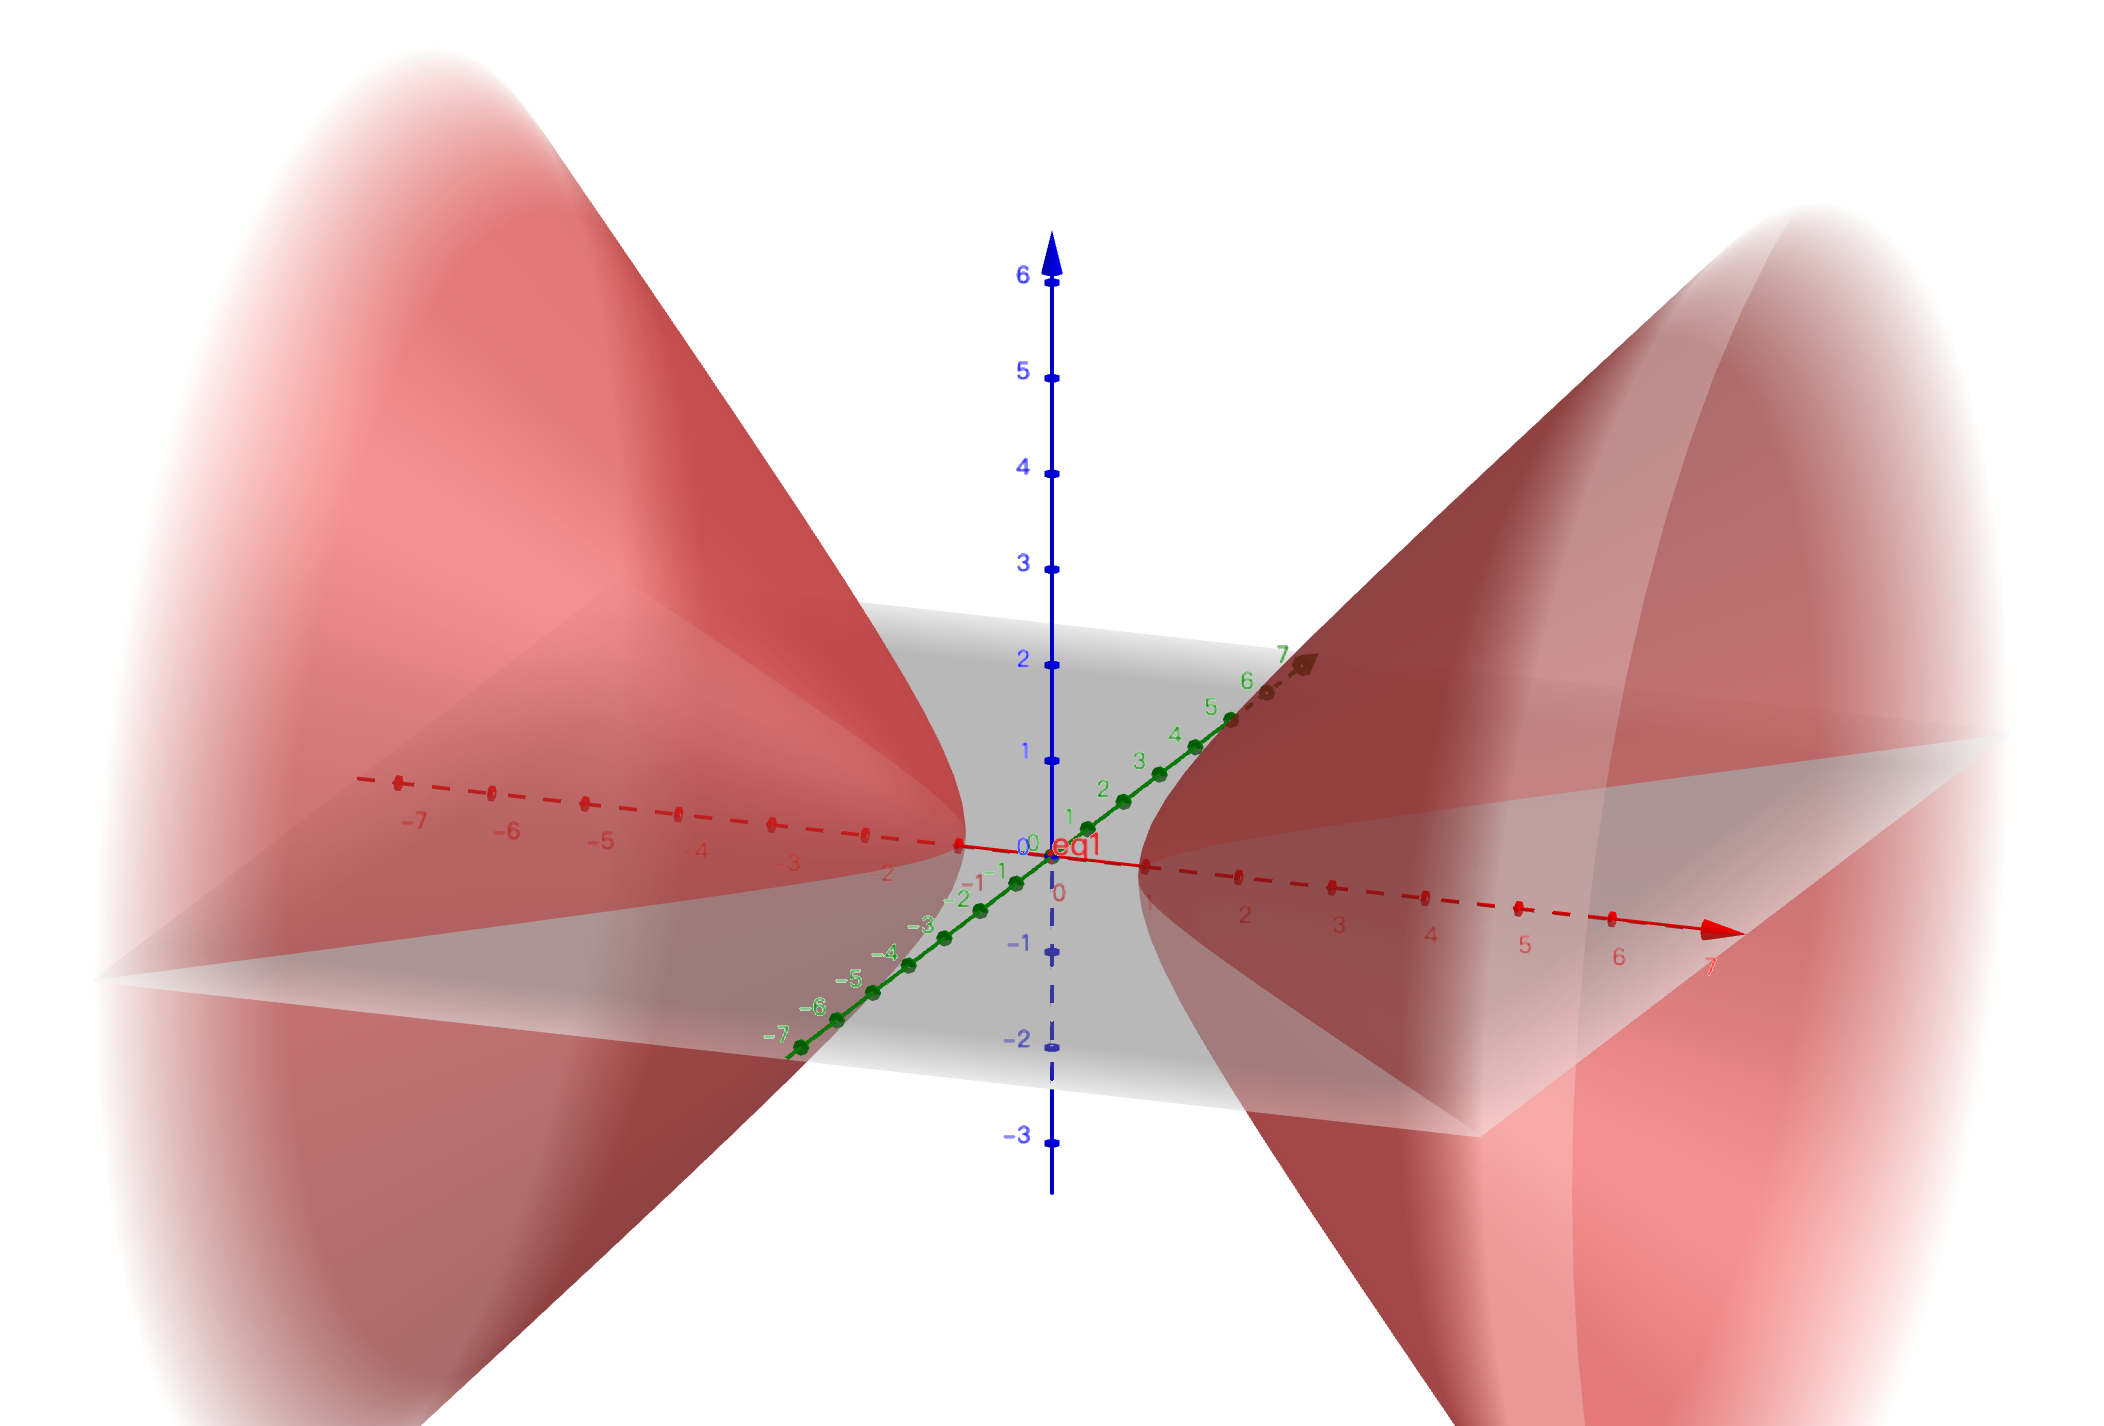
\includegraphics[scale=.2]{materials/1.png}
\end{center}
下面是 $x_1^2+x_2^2-x_3^2=1$ 的图象.
\begin{center}
    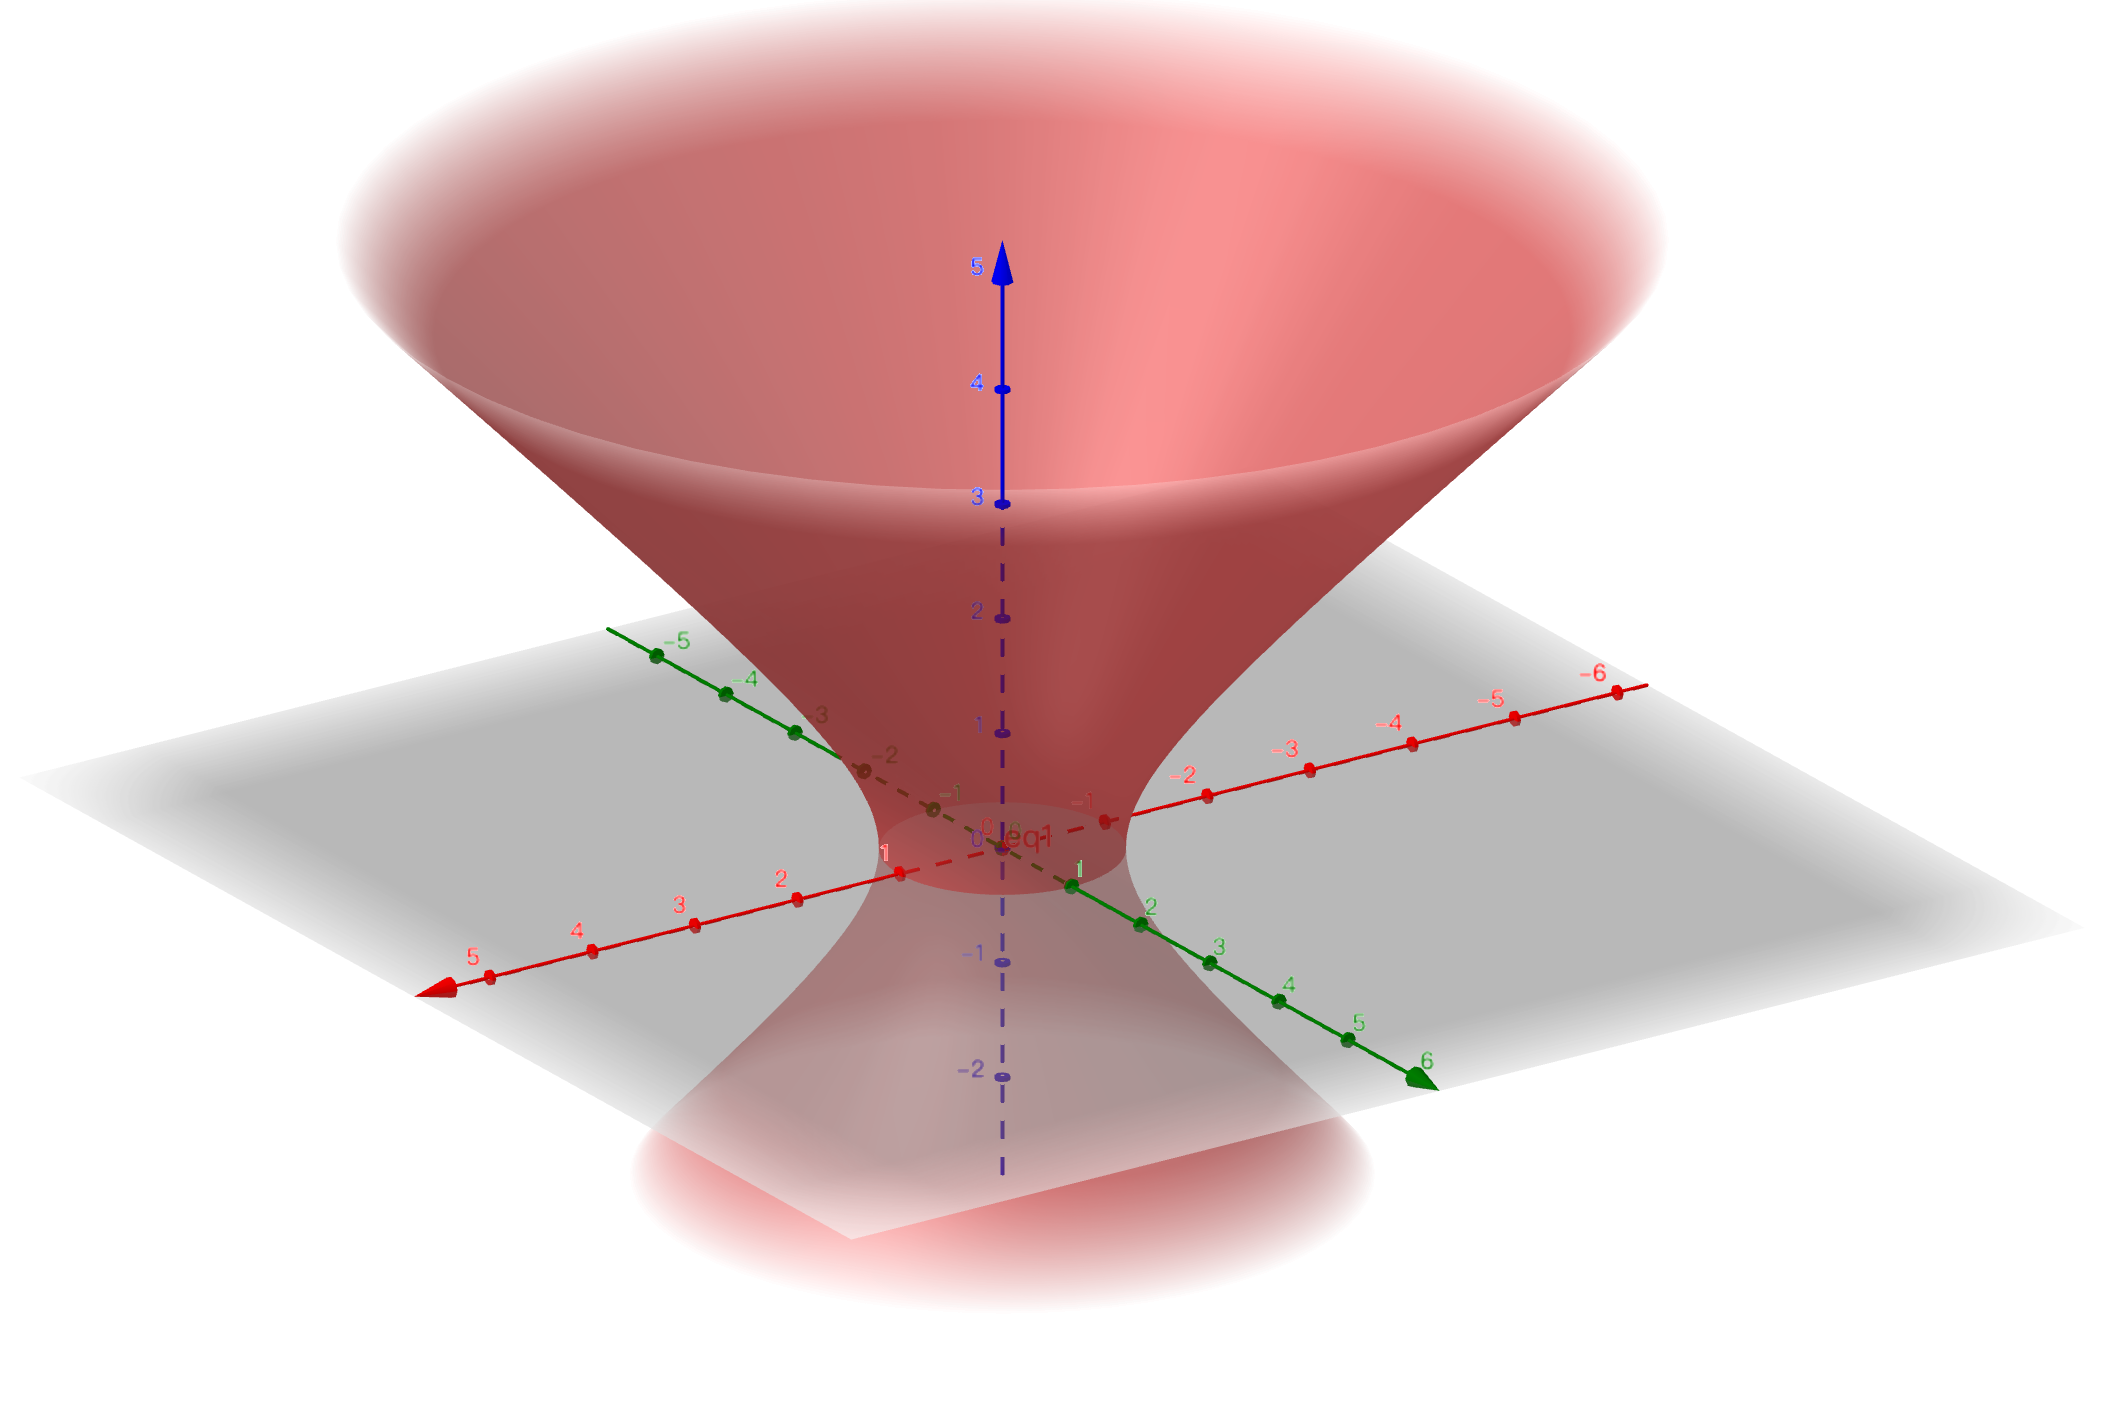
\includegraphics[scale=.2]{materials/2.png}
\end{center}
下面是 $x_1^2+x_2^2+2x_3=0$ 的图象.
\begin{center}
    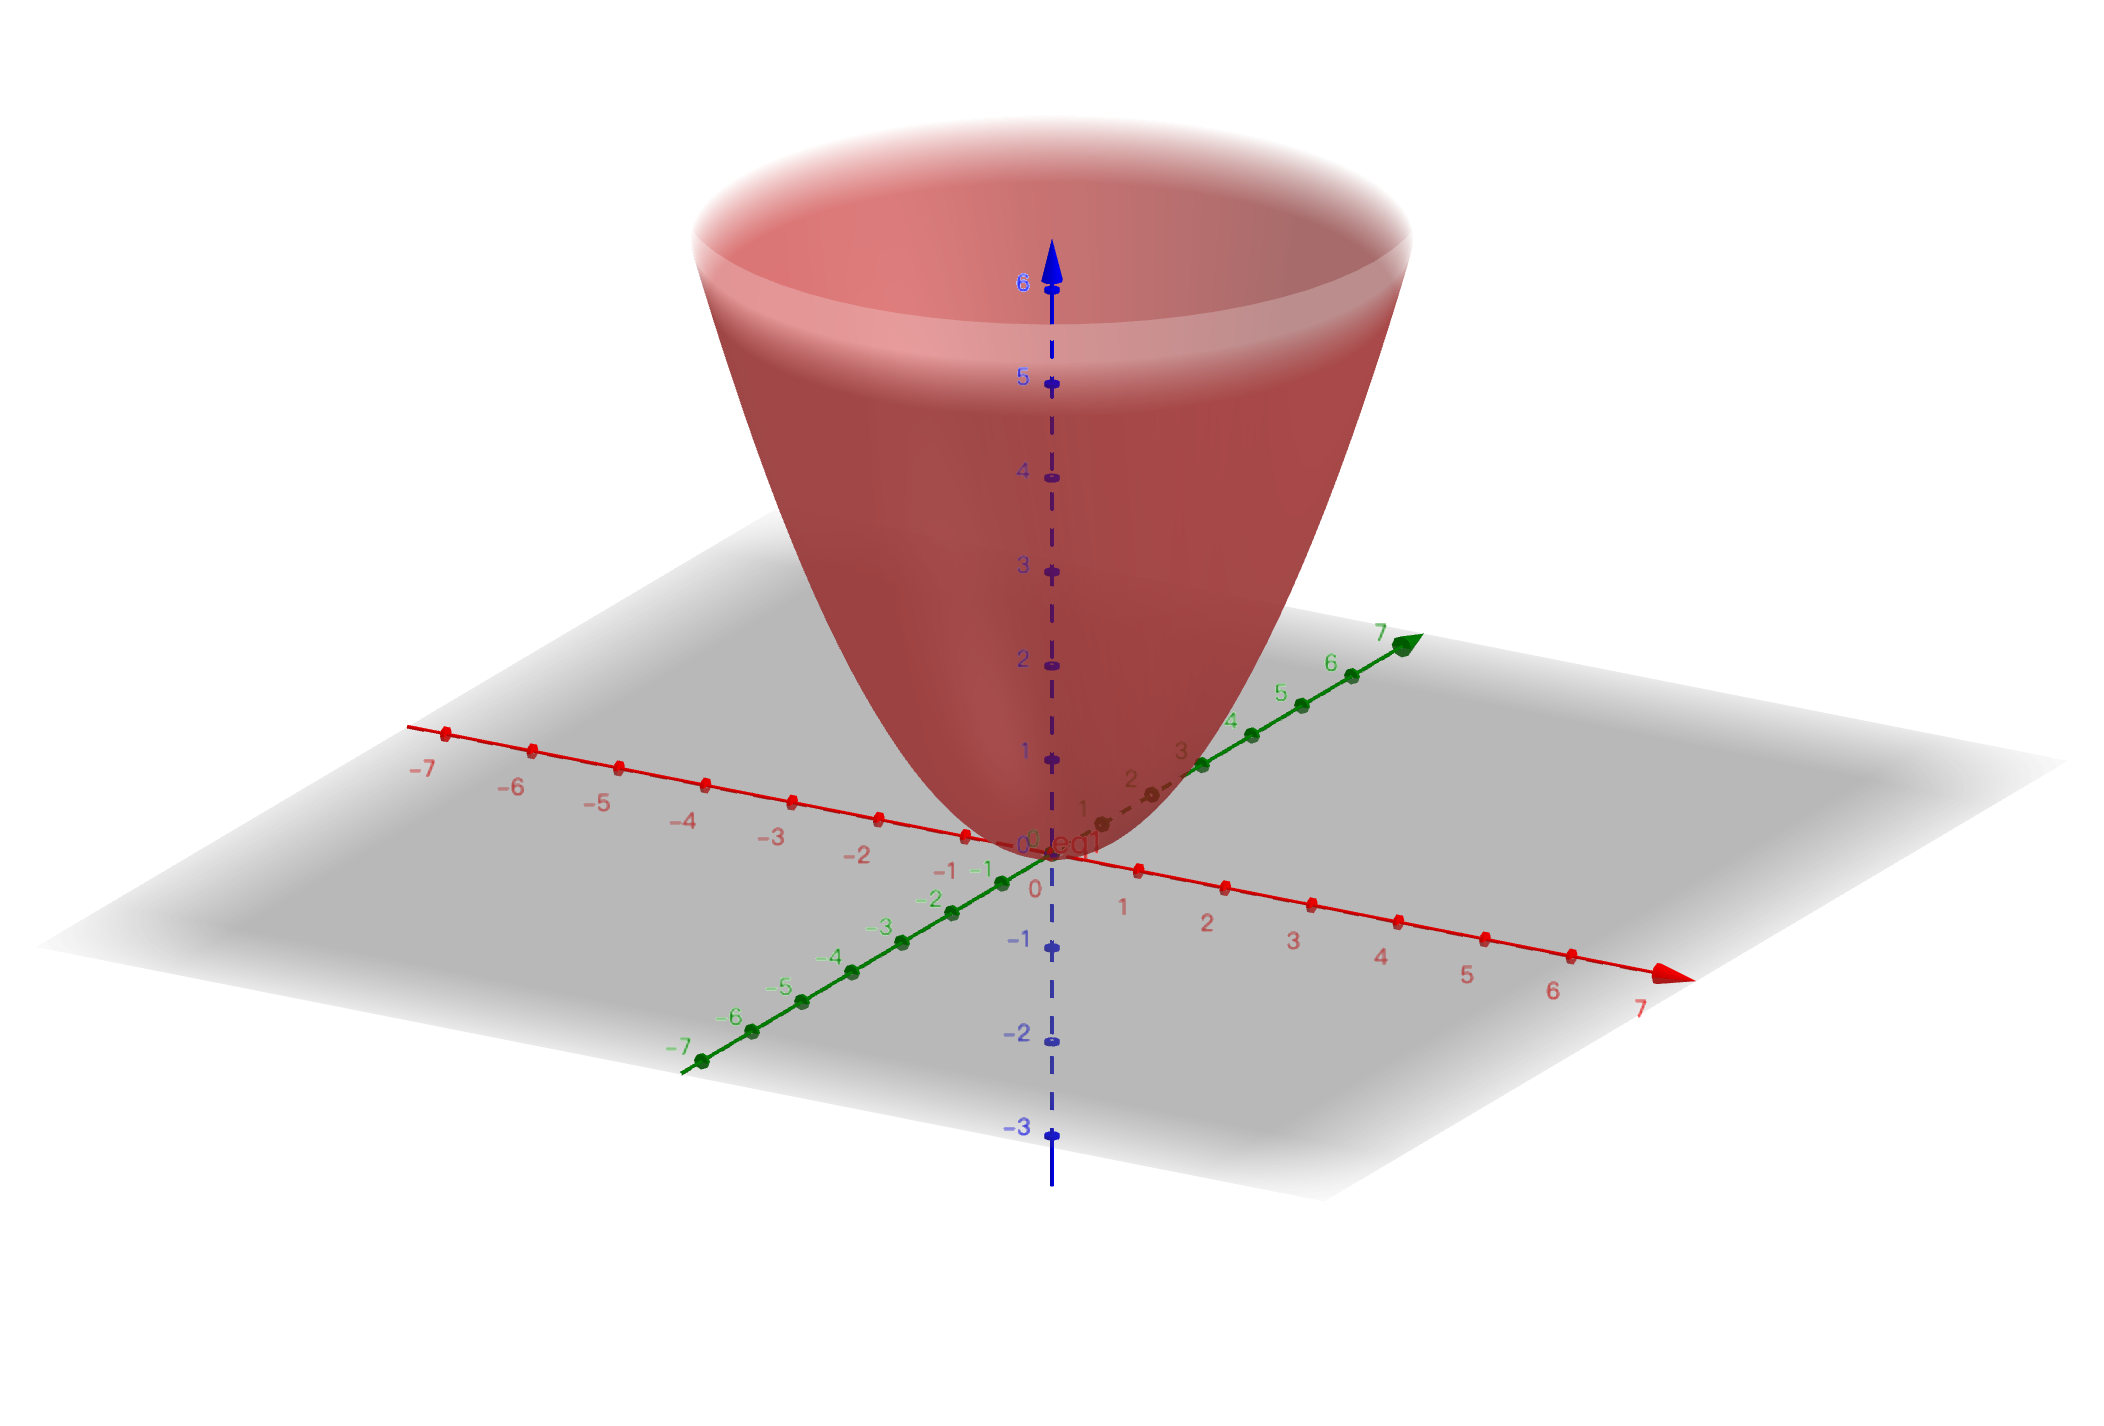
\includegraphics[scale=.2]{materials/3.png}
\end{center}
下面是 $x_1^2-x_2^2+2x_3=0$ 的图象.
\begin{center}
    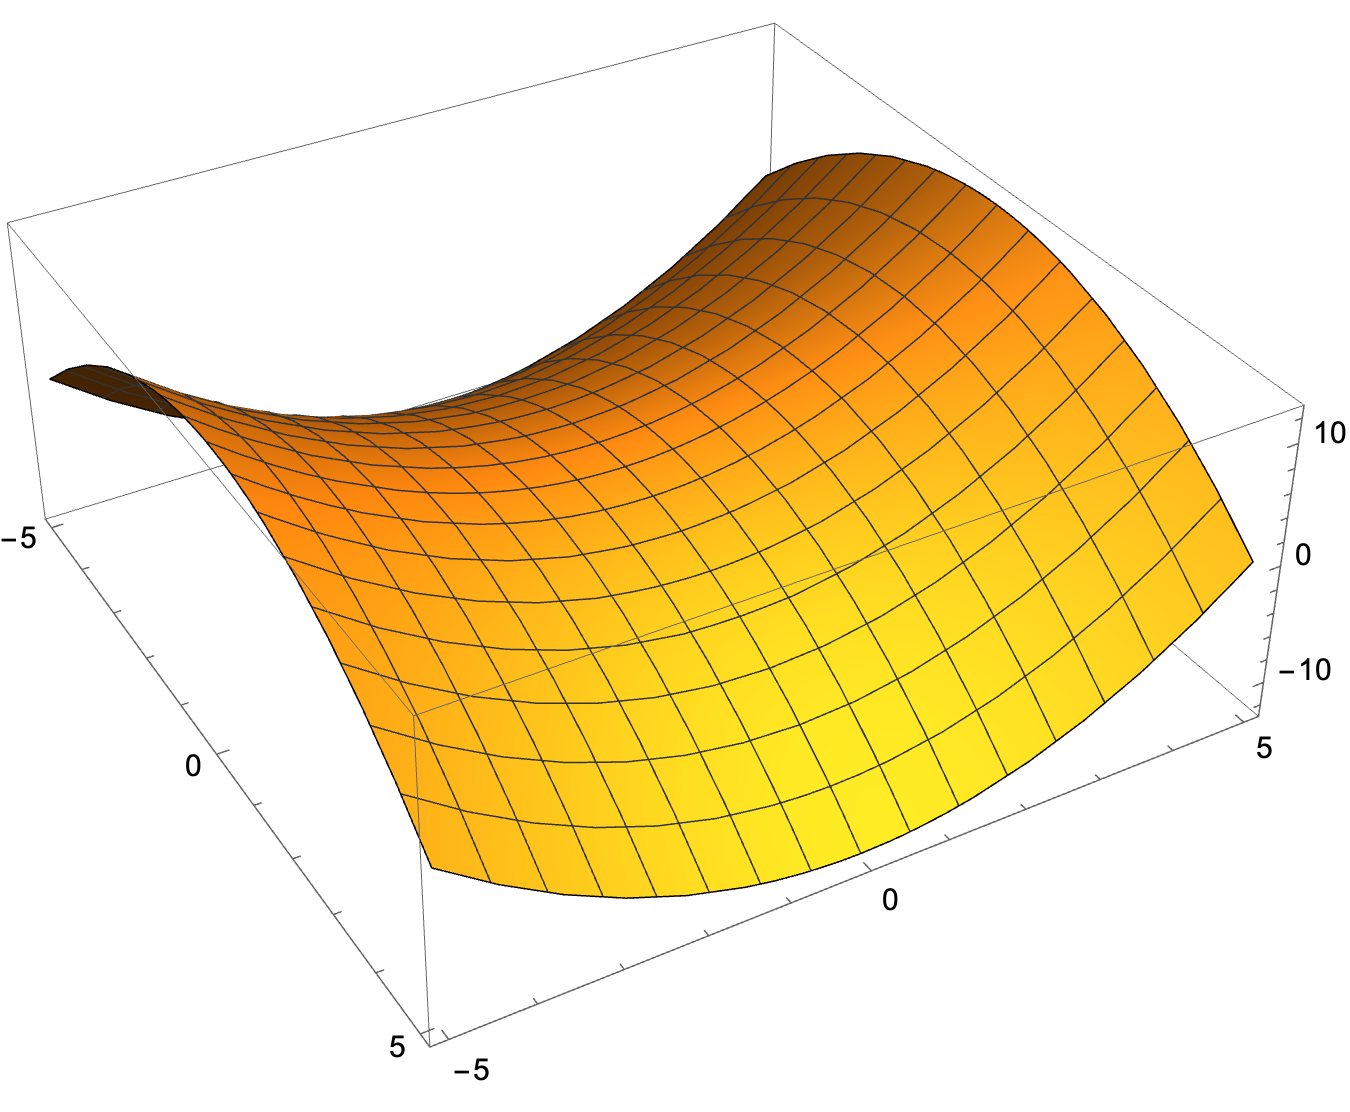
\includegraphics[scale=.5]{materials/4.png}
\end{center}
作为仿射空间中二次曲面的应用, 下面介绍\textbf{二次逼近}的概念.
\begin{example}
    设 $f(x_1,x_2,\cdots,x_n)$ 是多元函数, 由微积分中的 Taylor 定理, 可以用二次曲面
    \[f(x_1,\cdots,x_n)=f(0,\cdots,0)+\sum\limits_{i=1}^n\dfrac{\partial f}{\partial x_i}(0,\cdots,0)x_i+\dfrac{1}{2}\sum\limits_{1\leq i\leq j\leq n}\dfrac{\partial^2f}{\partial x_i\partial x_j}(0,\cdots,0)x_ix_j+R(x_1,\cdots,x_n)\]
    逼近 $f$.

    在 $n=2$ 的情形下将上式化为规范型:
    \[f=a+bx^2+cy^2.\]

    当 $b,c\geq0$ 时 $f$ 在 $(0,0)$ 处取极小值, 当 $b,c\leq0$ 时 $f$ 在 $(0,0)$ 处取极大值, 其余情况不确定.
\end{example}
\section{射影几何(对应第 3 节)}
\subsection{射影几何的构造}
用现代数学的观点来看待几何, 几何学的研究对象是 ``点'' 和 ``直线'' 等元素之间的关系而不是元素本身, ``点'' 和 ``直线'' 可以是任何东西而不会影响几何的模型.

下面我们来构造一个几何模型, 模型中的 ``点'' 是 $3$ 维向量空间 $\mathbb{R}^3$ (可以用一般的 $3$ 维向量空间代替)中的 $1$ 维子空间, ``直线'' 是 $\mathbb{R}^3$ 中的 $2$ 维子空间. ``点'' 与 ``直线'' 间的关系归结为 $\mathbb{R}^3$ 中 $1$ 维子空间和 $2$ 维子空间之间的关系. 有
\begin{theorem}
    上述几何模型满足 Euclid 几何的公理:

    (1) 不同的两点唯一确定一条直线. (2) 两条不同的直线交于唯一的一点.
\end{theorem}
\begin{proof}
    (1) 设 $l_1,l_2$ 是 $\mathbb{R}^3$ 的 $1$ 维子空间且 $l_1\neq l_2$. 设 $\boldsymbol{u}_1\in l_1\backslash\{\boldsymbol{0}\},\boldsymbol{u}_2\in l_2\backslash\{\boldsymbol{0}\}$, 则 $\boldsymbol{u}_1,\boldsymbol{u}_2$ 线性无关. $\therefore\left<l_1,l_2\right>=\left<\boldsymbol{u}_1,\boldsymbol{u}_2\right>$ 是 $2$ 维子空间. 由子空间的构造得直线是唯一的.

    (2) 设 $U_1,U_2$ 是 $\mathbb{R}^3$ 的 $2$ 维子空间. 如果 $U_1,U_2$ 不重合, 取 $\boldsymbol{x}\in U_1\backslash U_2$, 则 $U_1+U_2\supset U_2+\left<\boldsymbol{x}\right>=\mathbb{R}^3$. $\because U_1,U_2\subset\mathbb{R}^3\Rightarrow U_1+U_2\subset\mathbb{R}^3$, $\therefore U_1+U_2=\mathbb{R}^3$. $\therefore$
    \[\dim(U_1\cap U_2)=\dim U_1+\dim U_2-\dim(U_1+U_2)=1.\]

    若 $l_1,l_2\in U_1\cap U_2$, 则 $\dim l_1=\dim l_2=1,\left<l_1,l_2\right>\in U_1\cap U_2$. $\therefore\dim\left<l_1,l_2\right>=1$. $\therefore l_1$ 与 $l_2$ 重合.
\end{proof}
将这个几何模型称为\textbf{平面射影几何}. 称 $\mathbb{R}^3$ 中的 $2$ 维子空间全体为\textbf{射影平面}, 记作 $\mathbb{RP}^2$. 可以证明, 平面射影几何满足 Euclid 几何中除了平行公理之外的全部公理.

书上 P206 给出了平面射影几何的直观的模型. 这个模型给出了将无界的仿射平面加上无穷远直线映成一个有界的图形(一个紧集)的映射, 称这样的映射为\textbf{紧化}映射. 可以用 \verb|materials/2-5.ggb| 观察这个模型.

沿用书上 P206 后半部分的记号. $\sigma$ 准确的定义是
\[\sigma:\begin{array}{rcl}
    S^2_-\backslash S^1 & \to & \varPi \\
    \dot{p} & \to & \{\dot{o}+\lambda\overrightarrow{op}|\lambda\in K\}\cap\varPi \\
\end{array}.\]

有
\begin{lemma}\label{l3.1}
    $\sigma$ 是双射.
\end{lemma}
\begin{proof}
    对射影平面 $\varPi$ 上任一点 $\dot{q},\exists\dot{p}=\dot{o}+\dfrac{\overrightarrow{oq}}{\|\overrightarrow{oq}\|}\in S^2_-\backslash S^1$ 满足 $\dot{q}=\dot{o}+\|\overrightarrow{oq}\|\overrightarrow{op}$, 即 $\dot{q}=\sigma(\dot{p})$. $\therefore\sigma$ 是满射.
    
    设 $\dot{p}_1,\dot{p}_2\in S^2_-\backslash S^1$ 满足 $\sigma(\dot{p}_1)=\sigma(\dot{p}_2)=\dot{q}$, 则 $\dot{q}=\dot{o}+\lambda_1\overrightarrow{op_1}=\dot{o}+\lambda_2\overrightarrow{op_2}$. $\therefore\lambda_1\overrightarrow{op_1}=\lambda_2\overrightarrow{op_2}\Rightarrow|\lambda_1|\|\overrightarrow{op_1}\|=|\lambda_2|\|\overrightarrow{op_2}\|$.
    
    $\because\dot{p}_1,\dot{p}_2\in S^2$, $\therefore\|\overrightarrow{op_1}\|=\|\overrightarrow{op_2}\|=1$. $\therefore|\lambda_1|=|\lambda_2|$. $\because\dot{p}_1,\dot{p}_2\in S^2_-\backslash S^1$, $\therefore\overrightarrow{op_1},\overrightarrow{op_2}$ 的方向相同, $\therefore\lambda_1=\lambda_2\Rightarrow\overrightarrow{op_1}=\overrightarrow{op_2}\Rightarrow\dot{p}_1=\dot{p}_2$. $\therefore\sigma$ 是单射.
\end{proof}
\begin{theorem}
    $S^2_-\backslash S^1$ 上的两``直线''(大圆周与球面的交线) $l_1,l_2$ 在平面上的投影 $\sigma(l_1),\sigma(l_2)$ 平行(不包括重合的情形)当且仅当 $l_1\cap l_2\in S^1$.
\end{theorem}
\begin{proof}
    ($\Rightarrow$) 证明逆否命题. 设 $l_1\cap l_2=\dot{p}\in S^2_-\backslash S^1$, 则 $\sigma(\dot{p})=\sigma(l_1)\cap\sigma(l_2)$. $\therefore\sigma(l_1),\sigma(l_2)$ 不平行.
    
    ($\Leftarrow$) $\because l_1\cap l_2\in S^1,\therefore l_1\cap l_2\cap S^2_-=\varnothing$.

    假设 $\exists\dot{p}\in\sigma(l_1)\cap\sigma(l_2)$, 则 $\exists\dot{x}_1\in l_1,\dot{x}_2\in l_2$ 使得 $\sigma(\dot{x}_1)=\sigma(\dot{x}_2)=\dot{p}$. 由引理 \ref{l3.1} 得 $\dot{x}_1=\dot{x}_2$. $\therefore\dot{x}_1\in l_1\cap l_2\cap S^2_-$, 与 $l_1\cap l_2\cap S^2_-=\varnothing$ 矛盾. $\therefore\sigma(l_1)\cap\sigma(l_2)=\varnothing$, 即 $\sigma(l_1),\sigma(l_2)$ 平行.
\end{proof}
\begin{theorem}
    如果 $\dot{p},\dot{q},\dot{r}\in S^2_-\backslash S^1$, 那么 $\dot{p},\dot{q},\dot{r}$ 在同一个大圆周上当且仅当 $\sigma(\dot{p}),\sigma(\dot{q}),\sigma(\dot{r})$ 共线.
\end{theorem}
\begin{proof}
    设 $\sigma(\dot{p})=\dot{o}+\lambda_1\overrightarrow{op},\sigma(\dot{q})=\dot{o}+\lambda_1\overrightarrow{oq},\sigma(\dot{r})=\dot{o}+\lambda_1\overrightarrow{or}$, 则
    \[\sigma(\dot{q})-\sigma(\dot{p})=\lambda_2\overrightarrow{oq}-\lambda_1\overrightarrow{op},\quad\sigma(\dot{r})-\sigma(\dot{q})=\lambda_3\overrightarrow{or}-\lambda_2\overrightarrow{oq}.\]

    ($\Leftarrow$) $\because\sigma(\dot{p}),\sigma(\dot{q}),\sigma(\dot{r})$ 共线, $\therefore\exists\mu\in K$ 使得
    \begin{align*}
        & \sigma(\dot{q})-\sigma(\dot{p})=\mu(\sigma(\dot{r})-\sigma(\dot{q})) \\
        \Rightarrow\ & \lambda_3\overrightarrow{or}-\lambda_2\overrightarrow{oq}=\mu(\lambda_2\overrightarrow{oq}-\lambda_1\overrightarrow{op}) \\
        \Rightarrow\ & \overrightarrow{oq}=\dfrac{\lambda_3}{(\mu+1)\lambda_2}\overrightarrow{or}+\dfrac{\mu\lambda_1}{(\mu+1)\lambda_2}\overrightarrow{op}.
    \end{align*}

    $\therefore\overrightarrow{oq}\in\left<\overrightarrow{op},\overrightarrow{or}\right>$. $\therefore\dot{o},\dot{p},\dot{q},\dot{r}$ 在同一个平面上. $\because\dot{p},\dot{q},\dot{r}\in S^2_-\backslash S^1,\therefore\dot{p},\dot{q},\dot{r}$ 在同一个大圆周上.

    ($\Rightarrow$) 证明逆否命题. 设 $\left<\sigma(\dot{q})-\sigma(\dot{p}),\sigma(\dot{r})-\sigma(\dot{q})\right>=U$, 其中 $U$ 为 $\varPi$ 的方向子空间, 则 $\forall\dot{x}\in\varPi$, $\exists\mu_1,\mu_2$ 使得
    \begin{align*}
        \dot{x} & =\sigma(\dot{p})+\mu_1(\sigma(\dot{q})-\sigma(\dot{p}))+\mu_2(\sigma(\dot{r})-\sigma(\dot{q})) \\
        & =\sigma(\dot{p})+\mu_1(\lambda_2\overrightarrow{oq}-\lambda_1\overrightarrow{op})+\mu_2(\lambda_3\overrightarrow{or}-\lambda_2\overrightarrow{oq}) \\
        & =\sigma(\dot{p})+(\mu_1-\mu_2)\lambda_2\overrightarrow{oq}-\mu_1\lambda_1\overrightarrow{op}+\mu_2\lambda_3\overrightarrow{or} \\
        & =\dot{o}+(\mu_1-\mu_2)\lambda_2\overrightarrow{oq}+(1-\mu_1)\lambda_1\overrightarrow{op}+\mu_2\lambda_3\overrightarrow{or}.
    \end{align*}

    $\therefore\varPi\subset\dot{o}+\left<\overrightarrow{op},\overrightarrow{oq},\overrightarrow{or}\right>$.

    $\because\left<\sigma(\dot{q})-\sigma(\dot{p}),\sigma(\dot{r})-\sigma(\dot{q})\right>=U$, $\therefore\sigma(\dot{p}),\sigma(\dot{q}),\sigma(\dot{r})$ 不重合. $\therefore\sigma(\dot{p}),\sigma(\dot{q}),\sigma(\dot{r})$ 不全为球面与 $\varPi$ 的交点. 设 $\dot{p}\notin\varPi$.
    
    $\because\dot{p}\in\dot{o}+\left<\overrightarrow{op},\overrightarrow{oq},\overrightarrow{or}\right>$, $\therefore A(\dot{p},\varPi)\subset\dot{o}+\left<\overrightarrow{op},\overrightarrow{oq},\overrightarrow{or}\right>$. $\because\dim A(\dot{p},\varPi)=3$, $\therefore\dim\dot{o}+\left<\overrightarrow{op},\overrightarrow{oq},\overrightarrow{or}\right>=3$. $\therefore\dot{p},\dot{q},\dot{r}$ 不在同一个平面上. $\therefore\dot{p},\dot{q},\dot{r}$ 不在同一个大圆周上.
\end{proof}
\subsection{代数簇}
不加说明的话, 在后面的小节中, 设 $V$ 是无限域 $K$ 上的 $n$ 维向量空间, $\mathbb{P}(V)$ 是 $K$ 上的 $n$ 维射影空间.

为了与齐次坐标的性质
\[(\lambda\xi_0:\lambda\xi_1:\cdots:\lambda\xi_n)=(\xi_0:\xi_1:\cdots:\xi_n),\quad\forall\lambda\in K\]

相适应, 我们希望 $\mathbb{P}(V)$ 上的函数 $f$ 具有性质
\[f(\lambda\xi_0,\lambda\xi_1,\cdots,\lambda\xi_n)=f(\xi_0,\xi_1,\cdots,\xi_n),\quad\forall\lambda\in K.\]

在 $K[t_0,t_1,\cdots,t_n]$ 中, 只有常数函数满足上述性质. 但是可以将条件减弱为
\begin{equation}\label{eq3.1}
    f(\lambda\xi_0,\lambda\xi_1,\cdots,\lambda\xi_n)=0\Leftrightarrow f(\xi_0,\xi_1,\cdots,\xi_n)=0,\quad\forall\lambda\in K.
\end{equation}

容易验证, 任一齐次多项式 $f\in K[t_0,t_1,t_2,\cdots,t_n]$ 都满足上式. 进一步, 有
\begin{theorem}
    多项式 $f\in K[t_0,t_1,\cdots,t_n]$ 满足式 (\ref{eq3.1}) 当且仅当 $f$ 是齐次的.
\end{theorem}
\begin{proof}
    
\end{proof}
\begin{definition}
    称一些齐次多项式在 $\mathbb{P}(V)$ 中的公共零点组成的集合为一个\textbf{代数簇}(variety)或\textbf{代数流形}(manifold). 拓扑学中要求流形是光滑的, 所以一般称为代数簇.
\end{definition}
\begin{example}
    在 $\mathbb{P}(K^4)$ 中, $t_1^2+t_2^2+t_3^2+t_4^2+t_5^2=0$ 定义了一个(光滑的)代数簇. 当 $K=\mathbb{C}$ 时这个代数流形在弦论中有重要意义.
\end{example}
\begin{example}
    在 $\mathbb{P}(K^4)$ 中,
    \[\begin{cases}
        t_1^2+t_2^2+t_3^2+t_4^2+t_5^2=0 \\
        t_1t_2^2+t_2t_3^2=0 \\
    \end{cases}\]
    定义了一个代数簇.
\end{example}
\subsection{仿射图}
用下面的例子引出仿射图的概念.
\begin{example}
    射影空间 $\mathbb{RP}^1$ 是 $\mathbb{R}^2$ 中 $1$ 维子空间的集合. 设 $\boldsymbol{e}_1,\boldsymbol{e}_2$ 是 $\mathbb{R}^2$ 的一个基. 对 $\boldsymbol{v}=\alpha\boldsymbol{e}_1+\beta\boldsymbol{e}_2\in\mathbb{R}^2\backslash\{0\}$, $\tilde{v}\in\mathbb{RP}^1$ 的齐次坐标为 $(\alpha:\beta)$. $\because\forall\lambda\in\mathbb{R}\backslash\{0\},(\lambda\alpha:\lambda\beta)=(\alpha:\beta)$, $\therefore$ 齐次坐标不能唯一地表示 $\tilde{v}$.
    
    若 $\alpha\neq0$, 则 $(\alpha:\beta)=(1:\beta/\alpha)$. 坐标 $(1:\gamma)$ 在 $\gamma$ 取定后可以唯一地表示齐次坐标中第一个分量不为 $0$ 的子空间. $\therefore$ 设 $U_1=\{(\alpha:\beta)|\alpha\in\mathbb{R}\backslash\{0\}\}=\{(1:\gamma)|\gamma\in\mathbb{R}\}$, 则
    \[\begin{array}{rcl}
        U_1 & \to & \boldsymbol{e}_1+\mathbb{R}\boldsymbol{e}_2 \\
        (1:\gamma) & \to & \boldsymbol{e}_1+\gamma\boldsymbol{e}_2 \\
    \end{array}\]
    是双射.
    
    把 $\boldsymbol{e}_1$ 看成是 $\mathbb{R}^2$ 中的一个点, 则 $\boldsymbol{e}_1+\mathbb{R}\boldsymbol{e}_2$ 是仿射空间, 将其记作 $\mathbb{E}_1$. $\therefore\mathbb{RP}^1$ 的一个子集可以与仿射空间等同起来.

    同样地, 可以定义 $U_2=\{(\alpha:\beta)|\beta\neq0\}$, 则 $U_2$ 可以与仿射空间 $\mathbb{E}_2=\boldsymbol{e}_2+\mathbb{R}\boldsymbol{e}_1$ 等同起来.

    $\because\forall\boldsymbol{v}\in\mathbb{R}^2\backslash\{0\},\boldsymbol{v}$ 至少有一个坐标不为 $0$, $\therefore\mathbb{RP}^1=U_1\cap U_2$.

    $\because\mathbb{RP}^1\backslash U_1=\{(0:\beta)|\beta\in\mathbb{R}\}=\{(0:1)\}$. $\therefore\mathbb{RP}^1=U_1\cup\{(0:1)\}$. $\because$ 把 $(0:1)$ 写成 $(1:\alpha)$ 的形式, 就是 $\left(1:1\cdot\dfrac{1}{0}\right)=(1:\infty)$, $\therefore$ 可以认为 $(0:1)$ 是 $U_1$ 的无穷远点. 在书上 P207 的直观模型中, $(0:1)$ 是过点 $\dot{o}$ 的直径与圆的另一个交点.
\end{example}
对一般的射影空间 $\mathbb{P}(V)$, 设 $\boldsymbol{e}_0,\boldsymbol{e}_1,\cdots,\boldsymbol{e}_n$ 是 $V$ 的一个基, 令
\begin{align*}
    U_i & =\{(a_0:a_1:\cdots:a_n)|a_i\neq0,a_j\in K,j=0,1,\cdots,n\} \\
    & =\{(b_0:\cdots:b_{n-1}:1:b_{i+1}:\cdots:b_n)|b_j\in K,j=0,1,\cdots,n\},
\end{align*}

称形如仿射空间
\[\mathbb{E}_i=\boldsymbol{e}_i+\left<\boldsymbol{e}_0,\cdots,\widehat{\boldsymbol{e}}_i,\cdots,\boldsymbol{e}_n\right>\]
加上映射
\[\Phi_i:\begin{array}{rcl}
    U_i & \to & \mathbb{E}_i \\
    (b_0:\cdots:b_{n-1}:1:b_{i+1}:\cdots:b_n) & \to & b_0\boldsymbol{e}_0+\cdots+b_{i-1}\boldsymbol{e}_{i-1}+\boldsymbol{e}_i+b_{i+1}\boldsymbol{e}_{i+1}+\cdots+b_n\boldsymbol{e}_n \\
\end{array}\]
的结构为\textbf{仿射图}(chart).

对 $\forall\tilde{\boldsymbol{x}}=(a_0:a_1:\cdots:a_n)\in U_i$,
\[\Phi_i(\tilde{\boldsymbol{x}})=a_i^{-1}a_0\boldsymbol{e}_0+\cdots+\widehat{\boldsymbol{e}}_i+\cdots+a_i^{-1}a_n\boldsymbol{e}_n\in\mathbb{E}_i.\]

反之, 对 $\forall\boldsymbol{y}=a_i^{-1}a_0\boldsymbol{e}_0+\cdots+\widehat{\boldsymbol{e}}_i+\cdots+a_i^{-1}a_n\boldsymbol{e}_n\in\mathbb{E}_i,\exists\tilde{\boldsymbol{x}}=(a_0:\cdots:a_{i-1}:1:a_{i+1}:\cdots:a_n)\in U_i$ 使得 $\Phi_i(\tilde{\boldsymbol{x}})=\boldsymbol{y}$.

$\therefore\Phi_i(U_i)=\mathbb{E}_i$. $\because\Phi_i$ 是双射, $\therefore\Phi_i^{-1}$ 存在, $U_i=\Phi_i^{-1}(\mathbb{E}_i)$.

$\because\forall\tilde{\boldsymbol{x}}\in\mathbb{P}(V),\boldsymbol{x}\in V\backslash\{\boldsymbol{0}\}$, $\therefore\tilde{\boldsymbol{x}}$ 的坐标 $(a_0:a_1:\cdots:a_n)$ 中有非零项, 即 $\exists i$ 使得 $a_i\neq0$. $\therefore\tilde{\boldsymbol{x}}\in U_i$. $\therefore$
\[\mathbb{P}(V)=\bigcup\limits_{i=0}^nU_i=\bigcup\limits_{i=0}^n\Phi_i^{-1}(\mathbb{E}_i).\]

这说明射影空间是多个仿射图的并. 仿射图不是随便并起来的, 而是具有很好的组织方式. 仿射图类似于拼图\footnote{``chart'' 有拼图的意思}, 将所有仿射图拼起来可以得到整个射影空间. 与拼图不同的是, 仿射图之间可以有重合的部分.
\begin{example}\label{exa3.4}
    齐次多项式 $f(x_0,x_1,\cdots,x_n)$ 的零点定义了 $\mathbb{P}(V)$ 上的一个代数簇 $S$. 设 $S_0=\Phi_0(S\cap U_0)$, 则有 $S_0\subset\Phi_0(U_0)=\mathbb{E}_0$. 设 $\tilde{\boldsymbol{x}}=(a_0:a_1:\cdots:a_n)\in S\cap U_0$.
    
    $\because\tilde{\boldsymbol{x}}\in S$, $\therefore f(a_0,a_1,\cdots,a_n)=0$. $\because f$ 是齐次的, $\therefore f\left(1,\dfrac{a_1}{a_0},\dfrac{a_2}{a_0},\cdots,\dfrac{a_n}{a_0}\right)=0$.
    
    $\because\Phi_0(\tilde{\boldsymbol{x}})\in S_0$ 在以 $\boldsymbol{e}_0$ 为原点, $\boldsymbol{e}_1,\boldsymbol{e}_2,\cdots,\boldsymbol{e}_n$ 为基的坐标系下的坐标为 $\left(\dfrac{a_1}{a_0},\dfrac{a_2}{a_0},\cdots,\dfrac{a_n}{a_0}\right)$, $\therefore S_0$ 是 $\mathbb{E}_0$ 中多项式 $f(1,y_1,\cdots,y_n)$ 的零点集.

    反过来, 多项式函数 $g(y_1,y_2,\cdots,y_n)=0\ (\deg g=m)$ 定义了 $\mathbb{E}_0$ 上的一个曲面 $S_0$. 以 $\dfrac{x_i}{x_0}$ 代 $y_i$, 则
    \[f(x_0,x_1,x_2,\cdots,x_n)=x_0^mg\left(\dfrac{x_1}{x_0},\dfrac{x_2}{x_0},\cdots,\dfrac{x_n}{x_0}\right)\]
    是 $m$ 次齐次多项式. $\therefore f(x_0,x_1,x_2,\cdots,x_n)=0$ 定义了 $\mathbb{P}(V)$ 的一个代数簇 $S$. $\because g(x_1,x_2,\cdots,x_n)=f(1,x_1,x_2,\cdots,x_n)$, $\therefore\Phi_0(S\cap U_0)=S_0$.
\end{example}
例 \ref{exa3.4} 说明, 仿射空间中的曲面可以扩充为射影空间中的代数簇, 而 $\mathbb{P}(V)$ 是紧的, $\therefore$ 研究代数簇对研究仿射空间有重要意义.

举一个具体一点的例子.
\begin{example}
    考察 $\mathbb{P}(\mathbb{R}^2)$ 中的代数簇 $S:x_1^2+x_2^2=x_0^2$. $\Phi_0(S\cap U_0)$ 是 $\mathbb{E}_0$ 上的椭圆 $x_1^2+x_2^2=1$, $\Phi_1(S\cap U_1)$ 是 $\mathbb{E}_1$ 上的双曲线 $x_2^2=1+x_0^2$,
\end{example}

与 $2$ 维的情形类似, 有
\[\mathbb{P}(V)\backslash U_i=\{(\alpha_1:\cdots:\alpha_{i-1}:0:\alpha_{i+1}:\cdots:\alpha_n)\}=\{(\infty:\cdots:\infty:1(\text{第}i\text{个}):\infty:\cdots:\infty)\},\]

称 $\mathbb{P}(V)\backslash U_i$ 为 $U_i$ 的\textbf{无穷远空间}.

记 $\left<\boldsymbol{e}_0,\cdots,\widehat{\boldsymbol{e}}_i,\cdots,\boldsymbol{e}_n\right>=V_i$, 则有
\begin{theorem}
    $\mathbb{P}(V)\backslash U_i=\mathbb{P}(V_i)$.
\end{theorem}
\begin{proof}
    $\forall\tilde{\boldsymbol{u}}\in\mathbb{P}(V)\backslash U_i,\boldsymbol{u}=\alpha_1\boldsymbol{e}_1+\cdots+\hat{\boldsymbol{e}}_i+\cdots+\alpha_n\boldsymbol{e}_n\in V_i$, $\therefore\tilde{\boldsymbol{u}}\in\mathbb{P}(V_i)$. $\therefore\mathbb{P}(V)\backslash U_i\subset\mathbb{P}(V_i)$. 对称地, 有 $\mathbb{P}(V_i)\subset\mathbb{P}(V)\backslash U_i$.
\end{proof}
\subsection{射影群}
有两种看待射影空间 $\mathbb{P}(V)$ 的观点: $V$ 中 $1$ 维子空间全体和 $V^*/\sim$, 其中 $\boldsymbol{x}\sim\boldsymbol{y}\Leftrightarrow\exists\lambda,\boldsymbol{x}=\lambda\boldsymbol{y}$. 书上用第二种观点来定义射影变换, 其实用第一种观点来定义更为直观, 在处理一些问题的时候也更方便.

设 $\mathcal{A}\in\operatorname{GL}(V)$, 则 $\mathcal{A}$ 把 $V$ 中的 $1$ 维子空间映成 $1$ 维子空间. $\therefore$
\[\widetilde{\mathcal{A}}:\begin{array}{rcl}
    \mathbb{P}(V) & \to & \mathbb{P}(V) \\
    l & \to & \mathcal{A}l=\{\mathcal{A}\boldsymbol{x}|\boldsymbol{x}\in l\} \\
\end{array}\]
是确切定义的.

下面采用书上对 $\widetilde{\mathcal{A}}$ 的定义.
\begin{theorem}
    $\widetilde{\mathcal{A}}$ 是确切定义的.
\end{theorem}
\begin{proof}
    设 $\tilde{\boldsymbol{x}}=\tilde{\boldsymbol{y}}$, 则 $\exists\lambda\in K,\boldsymbol{x}=\lambda\boldsymbol{y}$. $\therefore\mathcal{A}\boldsymbol{x}=\mathcal{A}\lambda\boldsymbol{y}=\lambda\mathcal{A}\boldsymbol{y}$. $\therefore\widetilde{\mathcal{A}}\tilde{\boldsymbol{x}}=\widetilde{\mathcal{A}\boldsymbol{x}}=\widetilde{\mathcal{A}\boldsymbol{y}}=\widetilde{\mathcal{A}}\tilde{\boldsymbol{y}}$. $\therefore\widetilde{\mathcal{A}}$ 的值与代表元的选取无关.
\end{proof}
\begin{theorem}
    设仿射图 $\mathbb{E}_0=\boldsymbol{e}_0+\left<\boldsymbol{e}_1,\cdots,\boldsymbol{e}_n\right>$, 则映射
    \[\sigma:\begin{array}{rcl}
        \operatorname{Aff}(\mathbb{E}_0) & \to & \operatorname{PGL}(V) \\
        \tau & \to & \widetilde{\mathcal{A}} \\
    \end{array}\]
    是同态.
\end{theorem}
\begin{proof}
    设 $\mathbb{E}_0$ 中的点 $\dot{p}$ 在坐标系 $\{\boldsymbol{e}_0;\boldsymbol{e}_1,\cdots,\boldsymbol{e}_n\}$ 下的坐标为 $[x_1,x_2,\cdots,x_n]$, 可逆的仿射变换 $\tau$ 在坐标系 $\{\boldsymbol{e}_0;\boldsymbol{e}_1,\cdots,\boldsymbol{e}_n\}$ 下具有形式
    \[\tau(\dot{p})=A[x_1,x_2,\cdots,x_n]+[a_{10},\cdots,a_{n0}]\quad A=(a_{ij})\in\operatorname{GL}_n(K),a_{i0}\in K.\]

    设 $\tau(\dot{p})$ 在坐标系 $\{\boldsymbol{e}_0;\boldsymbol{e}_1,\cdots,\boldsymbol{e}_n\}$ 下的坐标为 $[y_1,y_2,\cdots,y_n]$, 则
    \[y_j=\sum\limits_{i=1}^na_{ij}x_i+a_{j0},\quad j=1,2,\cdots,n\]

    考虑 $V$ 上的线性算子
    \[\mathcal{A}:\begin{array}{rcl}
        \boldsymbol{e}_0 & \mapsto & \boldsymbol{e}_0 \\
        \boldsymbol{e}_i & \mapsto & \sum\limits_{i=1}^na_{ij}\boldsymbol{e}_i+a_{j0}\boldsymbol{e}_0\quad(i=1,2,\cdots,n) \\
    \end{array}.\]

    $\mathcal{A}$ 在基 $\boldsymbol{e}_0,\boldsymbol{e}_1,\cdots,\boldsymbol{e}_n$ 下的矩阵为
    \[\begin{pmatrix}
        1 & 0 \\
        A^{(0)} & A \\
    \end{pmatrix},\quad A^{(0)}=[a_{10},\cdots,a_{n0}].\]

    $\because A\in\operatorname{GL}_n(K)$, $\therefore\mathcal{A}$ 可逆. $\therefore\sigma$ 是确切定义的.

    设仿射变换 $\tau_1,\tau_2$ 在坐标系 $\{\boldsymbol{e}_0;\boldsymbol{e}_1,\cdots,\boldsymbol{e}_n\}$ 下具有形式
    \[\tau_1(\dot{p})=A_1[x_1,x_2,\cdots,x_n]+B_1\quad A_1\in\operatorname{GL}_n(K),B_1\in K^n,\]
    \[\tau_2(\dot{p})=A_2[x_1,x_2,\cdots,x_n]+B_2\quad A_2\in\operatorname{GL}_n(K),B_2\in K^n,\]

    则
    \[\tau_2\tau_1(\dot{p})=A_2A_1[x_1,x_2,\cdots,x_n]+A_2B_1+B_2.\]

    另一方面,
    \[\begin{pmatrix}
        1 & 0 \\
        B_2 & A_2 \\
    \end{pmatrix}\begin{pmatrix}
        1 & 0 \\
        B_1 & A_1 \\
    \end{pmatrix}=\begin{pmatrix}
        1 & 0 \\
        A_2B_1+B_2 & A_2A_1 \\
    \end{pmatrix},\]

    $\therefore\sigma(\tau_1\tau_2)=\sigma(\tau_1)\sigma(\tau_2)$, $\therefore\sigma$ 是同态.
\end{proof}
\subsection{射影几何的简单结论}
\begin{theorem}
    $\operatorname{PGL}(V)$ 可以把 $\mathbb{P}(V)$ 上的任意一点 $\tilde{x}$ 变为另一点 $\tilde{y}$.
\end{theorem}
\begin{proof}
    $\forall\boldsymbol{x},\boldsymbol{y}\in V\backslash\{0\}$, $\exists\mathcal{A}\in\operatorname{GL}(V)$ 使得 $\mathcal{A}\boldsymbol{x}=\boldsymbol{y}\Rightarrow\widetilde{\mathcal{A}}\tilde{\boldsymbol{x}}=\tilde{\boldsymbol{y}}$. 也可以由 $\widetilde{\mathcal{A}}$ 的双射性 (书上 P213) 得.
\end{proof}
\begin{theorem}
    设 $U$ 是 $V$ 的子空间, 则 $\widetilde{\mathcal{A}}\mathbb{P}(U)=\mathbb{P}(\mathcal{A}U)$ 是射影平面.
\end{theorem}
\begin{proof}
    
\end{proof}
\begin{theorem}
    射影空间中没有平行的概念.
\end{theorem}
\begin{proof}
    
\end{proof}
下面的性质是射影空间特有的, 在射影变换下不变的点比仿射空间的多一个.
\begin{theorem}[书上的定理 3]\label{t3.10}
    设 $\tilde{\boldsymbol{x}}_0,\tilde{\boldsymbol{x}}_1,\cdots,\tilde{\boldsymbol{x}}_{n+1}$ 和 $\tilde{\boldsymbol{y}}_0,\tilde{\boldsymbol{y}}_1,\cdots,\tilde{\boldsymbol{y}}_{n+1}$ 是处于一般位置的点组, 则 $\exists!\widetilde{\mathcal{A}}\in\operatorname{PGL}(V)$ 使得 $\widetilde{\mathcal{A}}\tilde{\boldsymbol{x}}_i=\tilde{\boldsymbol{y}_i},\ i=0,1,\cdots,n+1$.
\end{theorem}
\begin{proof}
    有
    \[\left<\boldsymbol{x}_1,\boldsymbol{x}_2,\cdots,\boldsymbol{x}_{n+1}\right>=V=\left<\boldsymbol{y}_1,\boldsymbol{y}_2,\cdots,\boldsymbol{y}_{n+1}\right>.\]

    $\therefore\exists\mathcal{B}\in\operatorname{GL}(V)$ 使得 $\mathcal{B}\boldsymbol{x}_i=\boldsymbol{y}_i,i=1,2,\cdots,n+1$. 然而不能保证有 $\mathcal{B}\boldsymbol{x}_0=\boldsymbol{y}_0$. 设
    \[\boldsymbol{x}_0=\sum\limits_{i=1}^{n+1}\alpha_i\boldsymbol{x}_i,\quad\boldsymbol{y}_0=\sum\limits_{i=1}^{n+1}\alpha_i\boldsymbol{y}_i.\]

    假设 $\exists\alpha_i=0$, 则有
    \[\boldsymbol{x}_0-(\alpha_1\boldsymbol{x}_1+\cdots+\alpha_{i-1}\boldsymbol{x}_{i-1}+\alpha_{i+1}\boldsymbol{x}_{i+1}+\cdots+\alpha_{n+1}\boldsymbol{x}_{n+1})=\boldsymbol{0},\]

    $\therefore\boldsymbol{x}_0,\cdots,\boldsymbol{x}_{i-1},\boldsymbol{x}_{i+1},\cdots,\boldsymbol{x}_{n+1}$ 线性相关.
    
    另一方面, $\because\tilde{\boldsymbol{x}}_0,\tilde{\boldsymbol{x}}_1,\cdots,\tilde{\boldsymbol{x}}_{n+1}$ 处于一般位置, $\therefore\boldsymbol{x}_0,\cdots,\boldsymbol{x}_{i-1},\boldsymbol{x}_{i+1},\cdots,\boldsymbol{x}_{n+1}$ 线性无关, 产生矛盾. $\therefore\alpha_i\neq0,\ i=1,2,\cdots,n+1$. 同理得 $\beta_i\neq0,\ i=1,2,\cdots,n+1$.
    
    定义
    \[\mathcal{C}:\boldsymbol{x}_i\to\dfrac{\beta_i}{\alpha_i}\boldsymbol{y}_i,\quad i=1,2,\cdots,n+1.\]

    $\because\beta_i\neq0,\ i=1,2,\cdots,n+1$, $\therefore\mathcal{C}\in\operatorname{GL}(V)$.

    考察 $\mathcal{A}=\mathcal{CB}\in\operatorname{GL}(V)$. 有 $\mathcal{A}\boldsymbol{x}_i=\lambda_i\boldsymbol{y}_i,\ i=1,2,\cdots,n+1$,
    \[\mathcal{A}\boldsymbol{x}_0=\mathcal{A}\sum\limits_{i=1}^{n+1}\alpha_i\boldsymbol{x}_i=\sum\limits_{i=1}^{n+1}\alpha_i\mathcal{A}\boldsymbol{x}_i=\sum\limits_{i=1}^{n+1}\alpha_i\lambda_i\boldsymbol{y}_i=\sum\limits_{i=1}^{n+1}\beta_i\boldsymbol{y}_i=\boldsymbol{y}_0.\]

    $\therefore\widetilde{\mathcal{A}}\tilde{\boldsymbol{x}}_i=\widetilde{\mathcal{A}\boldsymbol{x}_i}=\tilde{\boldsymbol{y}}_i,\ i=0,1,\cdots,n+1$.
\end{proof}
由书上定理 3 的推论, 在射影直线 $K\mathbb{P}^1$ 上去掉 $0,1,\infty$ 三个点和去掉任意的不重合的三个点是等价的. 研究 $K\mathbb{P}^1\backslash\{0,1,\infty\}$ 要比直接研究 $K\mathbb{P}^1$ 简单.

设 $\tilde{\boldsymbol{u}}_1,\tilde{\boldsymbol{u}}_2,\tilde{\boldsymbol{u}}_3$ 是 $K\mathbb{P}^1$ 上不重合的三个点. $\because\forall\sigma\in S_3,\tilde{\boldsymbol{u}}_1,\tilde{\boldsymbol{u}}_2,\tilde{\boldsymbol{u}}_3$ 与 $\tilde{\boldsymbol{u}}_{\sigma(1)},\tilde{\boldsymbol{u}}_{\sigma(2)},\tilde{\boldsymbol{u}}_{\sigma(3)}$ 间可以建立射影变换, $\therefore$ 在射影变换的意义下点组是没有顺序的. 这也可以从 $\mathbb{RP}^1$ 的直观模型看出.
\subsection{交比}
用子空间的观点来看射影空间 $\mathbb{P}(V)$. $V$ 中的四个共面但不重合的 $1$ 维子空间有公共点 $\boldsymbol{0}$. 古典几何中对平面上交于一点的四条直线有深入的研究. 如图 1, 考察直线 $u_1,u_2,u_3,u_4$ 被一直线 $l$ 截得的四点 $A,B,C,D$ 构成的线段的长度比.
\begin{figure}[ht!]
    \centering
    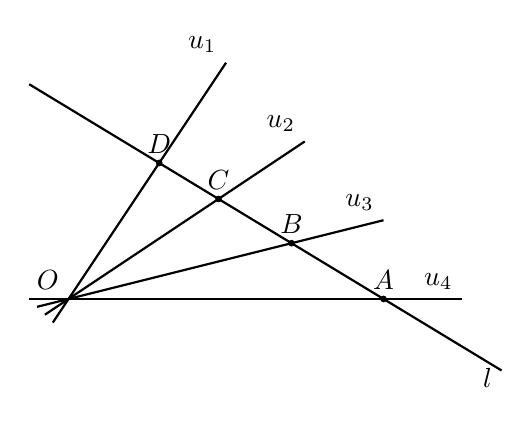
\begin{tikzpicture}
        \draw [thick] (-.2,-.3) -- (2,3);
        \node [above left] at (2,3) {$u_1$};
        \draw [thick] (-.3,-.2) -- (3,2);
        \node [above left] at (3,2) {$u_2$};
        \draw [thick] (-.4,-.1) -- (4,1);
        \node [above left] at (4,1) {$u_3$};
        \draw [thick] (-.5,0) -- (5,0);
        \node [above left] at (5,0) {$u_4$};
        \draw [thick] (-.5,0) -- (5,0);
        \node [above left] at (0,0) {$O$};
        \node [above] at (4,0) {$A$};
        \node [above] at (1.151,1.727) {$D$};
        \node [above] at (1.905,1.270) {$C$};
        \node [above] at (2.832,0.708) {$B$};
        \draw [fill] (4,0) circle (1pt);
        \draw [fill] (1.151,1.727) circle (1pt);        
        \draw [fill] (1.905,1.270) circle (1pt);        
        \draw [fill] (2.832,0.708) circle (1pt);
        \draw [thick,domain=-.5:5.5] plot(\x,{(--9.697-2.424*\x)/4});
        \node [left] at (5.5,-1) {$l$};
    \end{tikzpicture}
    \caption{交比的一个例子}
\end{figure}

只包括三个点的线段长度比, 比如 $\dfrac{AB}{AC}$, 在仿射变换下是不变的, 但在射影变换下会变化, 比如设 $C$ 是 $AB$ 的 $3$ 等分点, 则 $\exists$
\[\tilde{\mathcal{A}}:\begin{array}{rcl}
    A & \mapsto & B \\
    B & \mapsto & C \\
    C & \mapsto & A \\
\end{array},\]

将 $\dfrac{AB}{AC}$ 变为 $\dfrac{BC}{BA}=\dfrac{AB-BC}{AB}=1-\dfrac{AB}{AC}$.

古典几何中, 称
\[\dfrac{AC}{BC}\cdot\dfrac{BD}{AD}=\dfrac{AC}{BC}\cdot\left(\dfrac{AD}{BD}\right)^{-1}=\dfrac{AC}{BC}:\dfrac{AD}{BD}\]
为 $A,B,C,D$ 的\textbf{交比}, 记作 $[A,B,C,D]$.

将 $l$ 看成某个射影直线 $\mathbb{P}(U)\ (\dim U=2)$ 的仿射图 $(\mathbb{E}_0,\Phi_0)$, $A,B,C,D$ 在 $l$ 的一个坐标系 $\{\boldsymbol{e}_0;\boldsymbol{e}_1\}$ 下的坐标为 $x_1,x_2,x_3,x_4$, 则:
\[[A,B,C,D]=\dfrac{x_1-x_3}{x_2-x_3}\cdot\dfrac{x_2-x_4}{x_1-x_4}.\]

设 $\tilde{\boldsymbol{a}}=\Phi^{-1}_0(A)=\Phi^{-1}_0(\boldsymbol{e}_0+x_1\boldsymbol{e}_1),\tilde{\boldsymbol{b}}=\Phi^{-1}_0(B),\tilde{\boldsymbol{c}}=\Phi^{-1}_0(C),\tilde{\boldsymbol{d}}=\Phi^{-1}_0(D)$, 则有
\[[A,B,C,D]=[\tilde{\boldsymbol{a}},\tilde{\boldsymbol{b}},\tilde{\boldsymbol{c}},\tilde{\boldsymbol{d}}].\]

这说明古典几何中的交比是射影几何中的交比的一个特殊情况.

有
\begin{theorem}
    \[[A,B,C,D]=\dfrac{\sin\angle AOC}{\sin\angle BOC}\cdot\dfrac{\sin\angle BOD}{\sin\angle AOD}.\]
\end{theorem}
\begin{proof}
    如下图建立坐标系, 各点的坐标在点后, 则在坐标系 $\boldsymbol{e}_1,\boldsymbol{e}_2$ 下有 $\Phi_0^{-1}(A)=(s:x_1),\Phi_0^{-1}(B)=(s:x_2),\Phi_0^{-1}(C)=(s:x_3),\Phi_0^{-1}(D)=(s:x_4)$.
    \begin{figure}[h!]
        \centering
        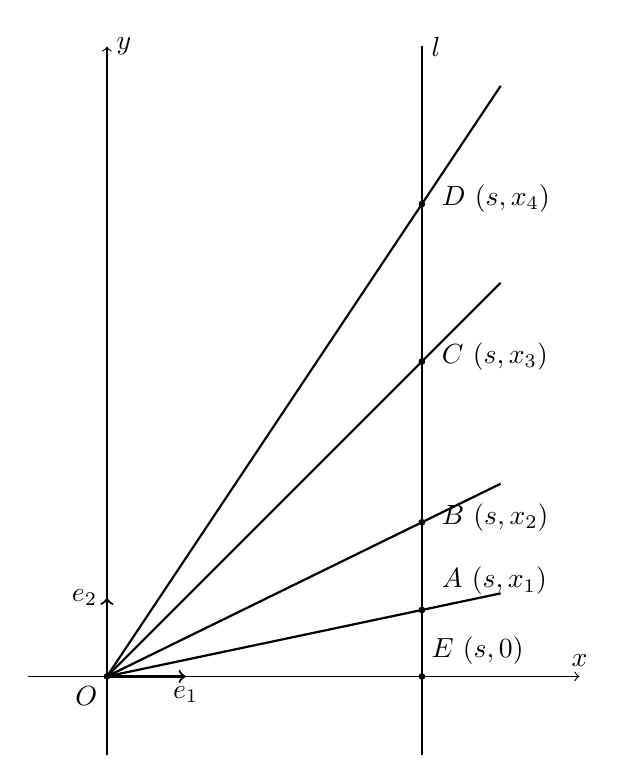
\begin{tikzpicture}
            \draw [->] (-1,0) -- (6,0);
            \draw [->] (0,-1) -- (0,8);
            \draw [thick, ->] (0,0) -- (1,0);
            \draw [thick, ->] (0,0) -- (0,1);
            \node [below] at (1,0) {$\boldsymbol{e}_1$};
            \node [left] at (0,1) {$\boldsymbol{e}_2$};
            \node [above] at (6,0) {$x$};
            \node [right] at (0,8) {$y$};
            \node [right] at (4,8) {$l$};
            \node [below left] at (0,0) {$O$};
            \draw [thick] (4,-1) -- (4,8);
            \draw [thick,domain=0:5] plot(\x,{(-0-0.844*\x)/-4});
            \draw [thick,domain=0:5] plot(\x,{(-0--1.958*\x)/4});
            \draw [thick,domain=0:5] plot(\x,{(-0--4*\x)/4});
            \draw [thick,domain=0:5] plot(\x,{(-0--6*\x)/4});
            \draw [fill] (4,0.8444838677059961) circle (1pt);
            \node [right] at (4.129,1.211) {$A\ (s,x_1)$};
            \draw [fill] (0,0) circle (1pt);
            \draw [fill] (4,1.958) circle (1pt);
            \node [below right] at (4.129,2.3182) {$B\ (s,x_2)$};
            \draw [fill] (4,4) circle (1pt);
            \node [below right] at (4.129,4.363) {$C\ (s,x_3)$};
            \draw [fill] (4,6) circle (1pt);
            \node [below right] at (4.129,6.373) {$D\ (s,x_4)$};
            \draw [fill] (4,0) circle (1pt);
            \node [right] at (4,0.325) {$E\ (s,0)$};
        \end{tikzpicture}
        \caption{交比不变性的证明}
    \end{figure}

    令 $\alpha=\angle AOE,\beta=\angle BOE,\gamma=\angle COE,\delta=\angle DOE$, 有
    \begin{align*}
        [A,B,C,D] & =[\Phi_0^{-1}(A),\Phi_0^{-1}(B),\Phi_0^{-1}(C),\Phi_0^{-1}(D)] \\
        & =\dfrac{\begin{vmatrix}
            s & x_1 \\
            s & x_3 \\
        \end{vmatrix}\cdot\begin{vmatrix}
            s & x_2 \\
            s & x_4 \\
        \end{vmatrix}}{\begin{vmatrix}
            s & x_1 \\
            s & x_4 \\
        \end{vmatrix}\cdot\begin{vmatrix}
            s & x_2 \\
            s & x_3 \\
        \end{vmatrix}} \\
        & =\dfrac{(x_3/s-x_1/s)(x_4/s-x_2/s)}{(x_4/s-x_1/s)(x_3/s-x_2/s)} \\
        & =\dfrac{(\tan\gamma-\tan\alpha)(\tan\delta-\tan\beta)}{(\tan\delta-\tan\alpha)(\tan\gamma-\tan\beta)} \\
        & =\dfrac{\left(\dfrac{\sin\gamma}{\cos\gamma}-\dfrac{\sin\alpha}{\cos\alpha}\right)\left(\dfrac{\sin\delta}{\cos\delta}-\dfrac{\sin\beta}{\cos\beta}\right)}{\left(\dfrac{\sin\delta}{\cos\delta}-\dfrac{\sin\alpha}{\cos\alpha}\right)\left(\dfrac{\sin\gamma}{\cos\gamma}-\dfrac{\sin\beta}{\cos\beta}\right)} \\
        & =\dfrac{(\sin\gamma\cos\alpha-\cos\gamma\sin\alpha)(\sin\delta\cos\beta-\cos\delta\sin\beta)}{(\sin\delta\cos\alpha-\cos\delta\sin\alpha)(\sin\gamma\cos\beta-\cos\gamma\sin\beta)} \\
        & =\dfrac{\sin(\gamma-\alpha)\sin(\delta-\beta)}{\sin(\delta-\alpha)\sin(\gamma-\beta)} \\
        & =\dfrac{\sin\angle AOC\sin\angle BOD}{\sin\angle AOD\sin\angle BOC}.\qedhere
    \end{align*}
\end{proof}
从上面的定理可以得到一些难以用古典方法得到的的结论, 比如对下图中的各点, 有 $[A,B,C,D]=[A',B',C',D']$.
\begin{figure}[h!]
    \centering
    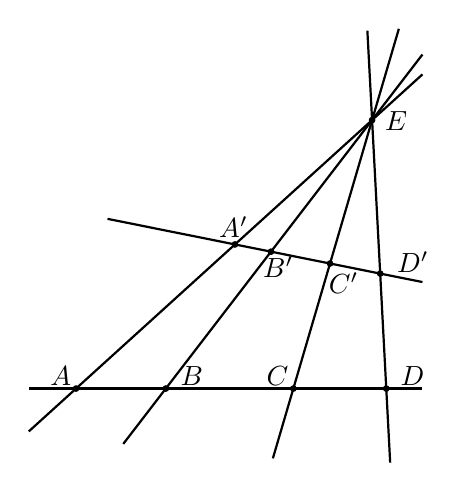
\begin{tikzpicture}
        \draw [thick,domain=0:5] plot(\x,{(--2.046-3.41*\x)/-3.76});
        \draw [thick,domain=1.2:5] plot(\x,{(--5.9334-3.41*\x)/-2.62});
        \draw [thick,domain=3.1:4.7] plot(\x,{(--11.4576-3.41*\x)/-1});
        \draw [thick,domain=4.3:4.59] plot(\x,{(--15.4814-3.41*\x)/0.18});
        \draw [thick,domain=1:5] plot(\x,{(-26.51371338752402--2.2585280618325987*\x)/-11.25307890380579});
        \draw [thick] (0,0) -- (5,0);
        \draw [fill] (0.6,0) circle (1pt);
        \node [left] at (0.6608960280884097,0.1612537565146532) {$A$};
        \draw [fill] (1.74,0) circle (1pt);
        \node [right] at (1.802993473655022,0.1612537565146532) {$B$};
        \draw [fill] (3.36,0) circle (1pt);
        \node [left] at (3.4197288186778887,0.1612537565146532) {$C$};
        \draw [fill] (4.54,0) circle (1pt);
        \node [right] at (4.598907350139521,0.1612537565146532) {$D$};
        \draw [fill] (4.36,3.41) circle (1pt);
        \node [right] at (4.4,3.4) {$E$};
        \draw [fill] (2.6184827203061456,1.8305920415542436) circle (1pt);
        \node [above] at (2.6,1.8) {$A'$};
        \draw [fill] (3.0759515392060566,1.7387766216384166) circle (1pt);
        \node [below] at (3.1675774345917533,1.8) {$B'$};
        \draw [fill] (3.8257727739865404,1.5882851592941016) circle (1pt);
        \node [below] at (4,1.6) {$C'$};
        \draw [fill] (4.462910933270255,1.4604095419357297) circle (1pt);
        \node [right] at (4.554410047065497,1.6074161064204247) {$D'$};
    \end{tikzpicture}
    \caption{交比的不变性}
\end{figure}
\begin{theorem}[书上的定理 5 的加强命题]
    设 $U$ 是 $2$ 维向量空间, 定点 $\tilde{\boldsymbol{a}}_1,\tilde{\boldsymbol{a}}_2,\tilde{\boldsymbol{a}}_3\in\mathbb{P}(U)$ 满足 $\tilde{\boldsymbol{a}}_1\neq\tilde{\boldsymbol{a}}_3,\tilde{\boldsymbol{a}}_2\neq\tilde{\boldsymbol{a}}_3$, 则 $[\tilde{\boldsymbol{a}}_1,\tilde{\boldsymbol{a}}_2,\tilde{\boldsymbol{a}}_3,\tilde{\boldsymbol{a}}_4]$ 可以唯一确定 $\tilde{\boldsymbol{a}}_4$.
\end{theorem}
\begin{proof}
    $\because\tilde{\boldsymbol{a}}_1,\tilde{\boldsymbol{a}}_3$ 两两不同, $\therefore U=\left<\boldsymbol{a}_1,\boldsymbol{a}_3\right>$.
    
    设 $\boldsymbol{a}_2=\mu\boldsymbol{a}_1+\nu\boldsymbol{a}_3$. 令 $\boldsymbol{e}=\mu\boldsymbol{a}_1,\boldsymbol{f}=\nu\boldsymbol{a}_3$, 则 $U=\left<\boldsymbol{e},\boldsymbol{f}\right>$. 在坐标系 $\boldsymbol{e},\boldsymbol{f}$ 下, $\tilde{\boldsymbol{a}}_1,\tilde{\boldsymbol{a}}_2,\tilde{\boldsymbol{a}}_3$ 的坐标分别为 $(1:0),(1,1),(0:1)$.
    
    设 $\tilde{\boldsymbol{a}}_4$ 在坐标系 $\boldsymbol{e},\boldsymbol{f}$ 下的坐标为 $(\alpha:\beta)$. $\because[\tilde{\boldsymbol{a}}_1,\tilde{\boldsymbol{a}}_2,\tilde{\boldsymbol{a}}_3,\tilde{\boldsymbol{a}}_4]$ 有定义, $\therefore\tilde{\boldsymbol{a}}_4\neq\tilde{\boldsymbol{a}}_1$, $\therefore\beta\neq0$. 代入书上的式 (19) 得
    \[[\tilde{\boldsymbol{a}}_1,\tilde{\boldsymbol{a}}_2,\tilde{\boldsymbol{a}}_3,\tilde{\boldsymbol{a}}_4]=\dfrac{\begin{vmatrix}
        1 & 0 \\
        0 & 1 \\
    \end{vmatrix}\cdot\begin{vmatrix}
        1 & 1 \\
        \alpha & \beta \\
    \end{vmatrix}}{\begin{vmatrix}
        1 & 0 \\
        \alpha & \beta \\
    \end{vmatrix}\cdot\begin{vmatrix}
        1 & 1 \\
        0 & 1 \\
    \end{vmatrix}}=1-\dfrac{\alpha}{\beta}.\]

    $\because\tilde{\boldsymbol{a}}_4$ 由 $\dfrac{\alpha}{\beta}$ 确定, $\therefore\tilde{\boldsymbol{a}}_4$ 由 $[\tilde{\boldsymbol{a}}_1,\tilde{\boldsymbol{a}}_2,\tilde{\boldsymbol{a}}_3,\tilde{\boldsymbol{a}}_4]$ 确定.
\end{proof}
设 $\tilde{\boldsymbol{a}}_1,\tilde{\boldsymbol{a}}_2,\tilde{\boldsymbol{a}}_3$ 和 $\tilde{\boldsymbol{b}}_1,\tilde{\boldsymbol{b}}_2,\tilde{\boldsymbol{b}}_3$ 是 $\mathbb{P}^1$ 上两两不同的点组, 由书上定理 3 的推论得 $\exists!\widetilde{\mathcal{A}}$ 使得 $\widetilde{\mathcal{A}}\tilde{\boldsymbol{a}}_i=\tilde{\boldsymbol{b}}_i\ (i=1,2,3)$.

一般地, 对于由 $[\tilde{\boldsymbol{a}}_1,\tilde{\boldsymbol{a}}_2,\tilde{\boldsymbol{a}}_3,\tilde{\boldsymbol{a}}_4],[\tilde{\boldsymbol{b}}_1,\tilde{\boldsymbol{b}}_2,\tilde{\boldsymbol{b}}_3,\tilde{\boldsymbol{b}}_4]$ 确定的 $\tilde{\boldsymbol{a}}_4,\tilde{\boldsymbol{b}}_4$, $\widetilde{\mathcal{A}}\tilde{\boldsymbol{a}}_4\neq\tilde{\boldsymbol{b}}_4$. 书上的定理 6 给出了 $\widetilde{\mathcal{A}}\tilde{\boldsymbol{a}}_4=\tilde{\boldsymbol{b}}_4$ 的充要条件.
\section{射影空间上的二次曲面(对应第 4 节)}
% 二次曲面-10 可以再看一遍, 可以听到很多故事
这节中, 设 $V$ 是 $\mathbb{R}$ 上的 $n+1$ 维线性空间.
\subsection{射影二次曲面的分类}
代数几何研究的是一些齐次多项式的零点集, 主要的问题是对这些集合分类. 射影几何中可以研究 $S=\{\tilde{\boldsymbol{u}}\in\mathbb{P}(V)|g_i(\tilde{\boldsymbol{u}})=0,i\in I\}$, 其中 $g_i$ 是 $\tilde{u}$ 的坐标的齐次多项式, $I\subset\mathbb{N}_+$ 是指标集. 定义 $\dim S=|I|$.

在高次数的情况下, 即使是 $1$ 维曲线都会非常复杂, 比如:
\begin{example}
    Fermat 大定理等价于: 齐次多项式
    \[x_1^n+x_2^n-x_3^n\in P(\mathbb{C}^3)\]

    在 $n\geq3$ 时的零点集为 $\{\boldsymbol{0}\}$.
\end{example}

下面只研究一个 $2$ 次多项式 $q$ 的零点集 $S_q=\{\tilde{\boldsymbol{u}}|q(\tilde{\boldsymbol{u}})=0\}$. 由书上第 1 章第 1 节定理 4 的推论 1\'(P34), $\exists V$ 的某个基 $\boldsymbol{e}_0,\boldsymbol{e}_1,\cdots,\boldsymbol{e}_n$, 使得 $q$ 在基 $\boldsymbol{e}_0,\boldsymbol{e}_1,\cdots,\boldsymbol{e}_n$ 下具有规范型
\[x^2_0+\cdots+x^2_s-x^2_{s+1}-\cdots-x^2_r.\]

$\because$
\[x^2_0+\cdots+x^2_s-x^2_{s+1}-\cdots-x^2_r=0,\quad -x^2_0-\cdots-x^2_s+x^2_{s+1}+\cdots+x^2_r=0\]
的解集相同, $\therefore$ 不妨设 $s\geq\left\lfloor\dfrac{r}{2}\right\rfloor$.

当 $s=r$ 时, 方程 $q(\tilde{\boldsymbol{u}})=0$ 只有零解, 这时在坐标 $(\boldsymbol{e}_i)$ 下有
\[S_q=\{(0:0:\cdots:0:x_{r+1}:\cdots:x_n)\}.\]

$\therefore S_q$ 是射影平面, 跟仿射空间的情形一样, 称其为\textbf{二重平面}. 也跟仿射空间的情形一样, 下面不加说明的话, 设 $s<r$.

以 $\dim V=4$ 的情况下的
\[\widetilde{C}:x_0^2+x_1^2+x_2^2-x_3^2=0\]
为例. 设 $\mathbb{E}_i=\boldsymbol{e}_i+V_i=\boldsymbol{e}_i+\left<\boldsymbol{e}_0,\cdots,\hat{\boldsymbol{e}}_i,\cdots,\boldsymbol{e}_3\right>$, 则 $\widetilde{C}\cap\mathbb{E}_i=\widetilde{C}_{i,a}$ ($a$ 表示仿射 affine)是仿射曲面. 具体地,

(i) $\widetilde{C}_{3,a}:x_0^2+x_1^2+x_2^2=1$ 是椭球面, $\widetilde{C}\cap\mathbb{P}(V_3):x_0^2+x_1^2+x_2^2=0$ 是空集.

(ii) $\widetilde{C}_{0,a}:x_3^2-x_1^2-x_2^2=1$ 是双叶双曲面, $\widetilde{C}\cap\mathbb{P}(V_0):x_3^2=x_1^2+x_2^2$ 是锥面. 由对称性, 与 $\mathbb{E}_1,\mathbb{E}_2$ 的交集跟与 $\mathbb{E}_0$ 的相同.

(iii) 作变换
\[\begin{cases}
    \beta_0=x_0 \\
    \beta_1=x_1 \\
    \beta_2=x_2-x_3 \\
    \beta_3=x_2+x_3 \\
\end{cases},\]

则
\[\widetilde{C}:\beta_0^2+\beta_1^2+\beta_2\beta_3=0.\]

在 $\beta_3=1$ 的仿射图中, $\widetilde{C}_a:\beta_0^2+\beta_1^2+\beta_2=0$ 是抛物面.

书上第 2 小节后面的部分可以总结为下面的定理. 这个定理说明, 可以像从一张二维的照片识别出三维物体一样通过与仿射图的交识别出射影二次曲面.
\begin{theorem}
    如果 $q(\tilde{\boldsymbol{u}})=0$ 定义的射影二次曲面 $\tilde{S}$ 不是二重平面, 且 $\tilde{S}\cap\mathbb{E}\neq\varnothing$, 那么 $\tilde{S}$ 完全由 $\mathbb{E}$ 确定.
\end{theorem}
\begin{proof}
    在代数几何的课程中会介绍下面证明的细节.

    $\because\mathbb{E}$ 是 $\mathbb{P}(V)$ 的开集, $\tilde{S}\cap\mathbb{E}\neq\varnothing$, $\therefore \tilde{S}\cap\mathbb{E}$ 是 $\tilde{S}$ 的开集.

    $\because \tilde{S}$ 是不可约代数簇, $\therefore\overline{\tilde{S}\cap\mathbb{E}}=\tilde{S}$.
\end{proof}
\begin{proof}[只用到现在所学知识的证明]
    设 $\mathbb{E}=\boldsymbol{e}+U$, 其中 $\dim U=n,\boldsymbol{e}\notin U$. 将 $\boldsymbol{e}$ 扩充为 $V$ 的一个基 $\boldsymbol{e}_0,\boldsymbol{e}_1,\cdots,\boldsymbol{e}_n$, 其中 $\boldsymbol{e}_0=\boldsymbol{e}$. 设 $S$ 在基 $\boldsymbol{e}_0,\boldsymbol{e}_1,\cdots,\boldsymbol{e}_n$ 下的方程为
    \[q(\boldsymbol{x})=\sum\limits_{i,j=1}^nf_{ij}x_ix_j,\]

    则 $\mathbb{E}$ 上的仿射二次曲面 $\tilde{S}\cap\mathbb{E}$ 在坐标系 $\{\boldsymbol{e};\boldsymbol{e}_1,\boldsymbol{e}_2,\cdots,\boldsymbol{e}_n\}$ 下的方程为
    \[q(\boldsymbol{e}+\boldsymbol{x})=\sum\limits_{i,j=1}^nf_{ij}x_ix_j+\sum\limits_{i=1}^nf_{0i}x_i+f_{00}.\]

    $\because\tilde{S}$ 不是二重平面, $\therefore q$ 在基 $\boldsymbol{f}_0,\boldsymbol{f}_1,\cdots,\boldsymbol{f}_n$ 下具有规范型
    \[y^2_0+\cdots+y^2_s-y^2_{s+1}-\cdots-y^2_r=0,\quad s<r,\]

    其中
    \[y_i=\sum\limits_{j=0}^na_{ij}x_j,\quad i=0,1,\cdots,n.\]

    $\therefore\tilde{S}\cap\mathbb{E}$ 在坐标系 $\{\boldsymbol{f}_0;\boldsymbol{f}_1,\boldsymbol{f}_2,\cdots,\boldsymbol{f}_n\}$ 下的方程为
    \[q(\boldsymbol{f}_0+\boldsymbol{x})=x^2_0+\cdots+x^2_s-x^2_{s+1}-\cdots-x^2_r=0.\]

    $\because s<r$, $\therefore\tilde{S}\cap\mathbb{E}$ 不是二重平面.

    如果有 $q'$ 使得 $q'(\boldsymbol{e}+\boldsymbol{u})=0$ 与 $\tilde{S}\cap\mathbb{E}$ 重合, 由书上第 2 节的定理 1 得 $q'=\lambda q,\lambda\in\mathbb{R}$. $\therefore q'(\tilde{\boldsymbol{x}})=\lambda q(\tilde{\boldsymbol{x}})$, 即两曲面相等.
\end{proof}
\subsection{切线与切面}
设直线 $l$ 经过 $\tilde{\boldsymbol{a}}=(a_0:a_1:\cdots:a_n),\tilde{\boldsymbol{b}}=(b_0:b_1:\cdots:b_n)$ 两点, 则 $l=\mathbb{P}(\left<\boldsymbol{a},\boldsymbol{b}\right>)$ 上的点可以表示为
\[(\lambda a_0+\mu b_0:\lambda a_1+\mu b_1:\cdots:\lambda a_n+\mu b_n),\quad\lambda,\mu\in\mathbb{R},\lambda^2+\mu^2\neq0.\]

不妨设 $\mu\neq0,x=\dfrac{\lambda}{\mu}$, 则 $l$ 上的点可以表示为
\[(xa_0+b_0:xa_1+b_1:\cdots:xa_n+b_n),\quad x\in\mathbb{R}\backslash\{0\}.\]

设 $S:q(\tilde{\boldsymbol{u}})=0$, $f$ 是与 $q$ 配极的双线性型, 设 $\tilde{\boldsymbol{u}}\in l\cap S$, 则
\[q(\boldsymbol{u})=f(\boldsymbol{u},\boldsymbol{u})=f(x\boldsymbol{a}+\boldsymbol{b},x\boldsymbol{a}+\boldsymbol{b})=x^2q(\boldsymbol{a})+2xf(\boldsymbol{a},\boldsymbol{b})+q(\boldsymbol{b}).\]

$\because\tilde{\boldsymbol{u}}\in S$, $\therefore$
\begin{equation}\label{eq4.1}
    x^2q(\boldsymbol{a})+2xf(\boldsymbol{a},\boldsymbol{b})+q(\boldsymbol{b})=0.
\end{equation}

如果 $f(\boldsymbol{a},\boldsymbol{b})=q(\boldsymbol{a})=q(\boldsymbol{b})=0$, 则 $\forall x$, 方程 \ref{eq4.1} 都成立. $\therefore l\in S$, 即 $l$ 是 $S$ 的母线. 下面设 $f(\boldsymbol{a},\boldsymbol{b}),q(\boldsymbol{a}),q(\boldsymbol{b})$ 不全为 $0$.

如果 $4f(\boldsymbol{a},\boldsymbol{b})-4q(\boldsymbol{a})q(\boldsymbol{b})=0$, 那么方程 \ref{eq4.1} 有二重解.

类比 Euclid 空间中曲线与直线相交的情况 (如下图, 下图也可以看成是 $\mathbb{RP}^1$ 的情形). Euclid 空间中把直线方程代入曲线方程后得到二重解等价于直线与曲线相切. $\therefore$ 可以将方程 \ref{eq4.1} 有二重解定义为 $S$ 与 $l$ 相切与 $\tilde{\boldsymbol{u}}$.
\begin{figure}[h!]
    \centering
    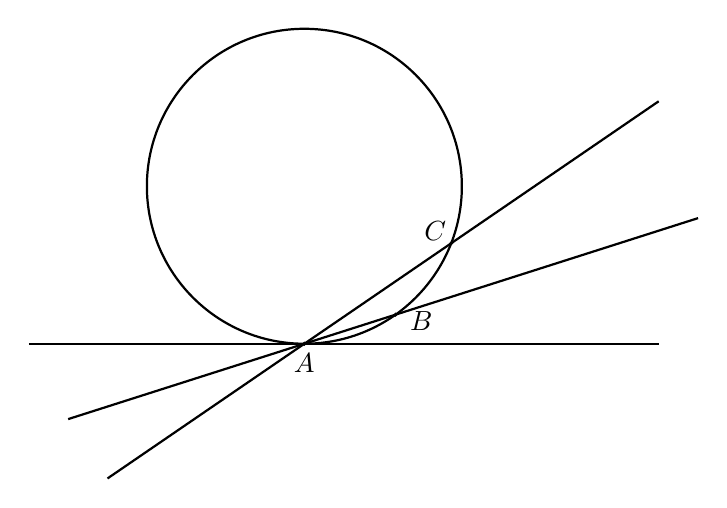
\begin{tikzpicture}[scale=.5]
        \draw [thick] (0,4) circle (4cm);
        \draw [thick, domain=-5:9] plot(\x,{(-0--2.551*\x)/3.728});
        \draw [thick, domain=-6:10] plot(\x,{(-0--0.739*\x)/2.316});
        \draw [thick, domain=-7:9] plot(\x,{(-0-0*\x)/-4});
        \draw [fill] (0,0) circle (1pt);
        \node [below] at (0,0) {$A$};
        \draw [fill] (3.728,2.551) circle (1pt);
        \node [left] at (3.846,2.871) {$C$};
        \draw [fill] (2.316,0.739) circle (1pt);
        \node [below right] at (2.438,1.066) {$B$};
    \end{tikzpicture}
    \caption{曲线与直线相交或相切}
\end{figure}

跟仿射曲面的情形一样, 定义
\begin{definition}
    对任意曲面 $S$, 设 $\tilde{\boldsymbol{p}}=(x_0:x_1:\cdots:x_n)\in S$. 如果
    \[\dfrac{\partial q}{\partial x_i}\Bigg|_{\tilde{\boldsymbol{p}}}=0,\quad i=0,1,\cdots,n,\]

    则称 $\tilde{\boldsymbol{p}}$ 是\textbf{奇点}. 如果 $\tilde{\boldsymbol{p}}$ 不是奇点, 则过 $\tilde{\boldsymbol{p}}$ 可以作 $S$ 的\textbf{切平面}:
    \[\sum\limits_{i=0}^n\left(\dfrac{\partial q}{\partial x_i}\bigg|_{\tilde{\boldsymbol{p}}}\right)\cdot x_i=0.\]
\end{definition}
% 特别地, 对仿射二次曲面
% \[q(\boldsymbol{x})=\sum\limits_{i,j=0}^nf_{ij}x_ix_j=0,\quad f_{ij}=f_{ji},\]

% 有
% \[\dfrac{\partial q}{\partial x_i}=2\sum\limits_{i=0}^nf_{ij}x_ix_j\]

对 $\mathbb{P}(V)$ 的仿射图 $\mathbb{E}$, $S\cap\mathbb{E}$ 的切线和切面是有定义的. 我们希望 $S$ 的切线和切面的定义与 $S\cap\mathbb{E}$ 的切线和切面的定义是相容的. 第 \ref{exc1} 题(在 $S$ 是二次曲面的情形下)证明了这个设想.
\section{第 5 章习题}
\subsection{习题 5.1}
\begin{exercise}[1.1]
    设 $2s\geq r>0$, 找出在 $n$ 维的实仿射空间上秩为 $r$ 的, 中心的二次函数 $Q$ 的等价类的个数.
\end{exercise}
\begin{solution}
\end{solution}
\begin{exercise}[1.2]
    求出在域 $\mathbb{R}$ 上的仿射空间上的二次函数
    \[Q(\boldsymbol{x})=x_1^2+2\sum\limits_{1\leq i<j\leq n}x_ix_j+2\sum\limits_{i=1}^nx_i+1\]

    的中心集 $C(Q)$.
\end{exercise}
\begin{solution}
    问题等价于求方程
    \[\begin{pmatrix}
        1 & 1 & 1 & \cdots & 1 & 1 \\
        1 & 0 & 1 & \cdots & 1 & 1 \\
        1 & 1 & 0 & \cdots & 1 & 1 \\
        \vdots & \vdots & \vdots & \ddots & \vdots & \vdots \\
        1 & 1 & 1 & \cdots & 0 & 1 \\
        1 & 1 & 1 & \cdots & 1 & 0 \\
    \end{pmatrix}X+\begin{pmatrix}
        2 \\
        2 \\
        \vdots \\
        2 \\
    \end{pmatrix}=0\]
    的解集. 解得 $C(Q)=\{(-2,0,0,\cdots,0)\}$.
\end{solution}
\subsection{习题 5.2}
\begin{exercise}[2.2]
    给出直角坐标系 $\{\dot{o},\boldsymbol{e}_1,\boldsymbol{e}_2,\boldsymbol{e}_3\}$, 将下列 $\mathbb{E}$ 中的二次曲面的二次部分化到主轴上:
    \begin{align*}
        (1) &\ Q([x,y,z])=2x^2+y^2-3z^2+12xy+4xz+8yz+18=0; \\
        (2) &\ Q([x,y,z])=6x^2+5y^2+7z^2+4xy-4xz-8x-10y+14z-6=0. \\
    \end{align*}
\end{exercise}
\begin{solution}
    (1) 二次方程的二次部分在 $\boldsymbol{e}_1,\boldsymbol{e}_2,\boldsymbol{e}_3$ 下的矩阵为
    \[\begin{pmatrix}
        2 & 6 & 2 \\
        6 & 1 & 4 \\
        2 & 4 & -3 \\
    \end{pmatrix},\]

    特征多项式为
    \[\begin{vmatrix}
        t-2 & -6 & -2 \\
        -6 & t-1 & -4 \\
        -2 & -4 & t+3 \\
    \end{vmatrix}=t^3-63t-162=(t-9)(t+3)(t+6),\]

    特征值为 $9,-3,-6$, 对应的特征向量为
    \[\begin{pmatrix}
        2 \\
        2 \\
        1 \\
    \end{pmatrix},\quad\begin{pmatrix}
        -2 \\
        1 \\
        2 \\
    \end{pmatrix},\quad\begin{pmatrix}
        1 \\
        -2 \\
        2 \\
    \end{pmatrix},\]

    $\therefore$ 在直角坐标系 $\{\dot{o},2\boldsymbol{e}_1+2\boldsymbol{e}_2+\boldsymbol{e}_3,-2\boldsymbol{e}_1+\boldsymbol{e}_2+2\boldsymbol{e}_3,\boldsymbol{e}_1-2\boldsymbol{e}_2+\boldsymbol{e}_3\}$ 下有
    \[Q([x,y,z])=9x^2-3y^2-6z^2+18.\]

    (2) 二次方程的二次部分 $q$ 在 $\boldsymbol{e}_1,\boldsymbol{e}_2,\cdots,\boldsymbol{e}_n$ 下的矩阵为
    \[\begin{pmatrix}
        6 & 2 & -2 \\
        2 & 5 & 0 \\
        -2 & 0 & 7 \\
    \end{pmatrix},\]

    特征值为 $9,6,3$, 对应的特征向量为
    \[\begin{pmatrix}
        -2 \\
        -1 \\
        2 \\
    \end{pmatrix},\quad\begin{pmatrix}
        1 \\
        2 \\
        2 \\
    \end{pmatrix},\quad\begin{pmatrix}
        2 \\
        -2 \\
        1 \\
    \end{pmatrix},\]

    $\therefore$ 在标准正交基 $\boldsymbol{v}_1=-2\boldsymbol{e}_1-\boldsymbol{e}_2+2\boldsymbol{e}_3,\boldsymbol{v}_2=\boldsymbol{e}_1+2\boldsymbol{e}_2+2\boldsymbol{e}_3,\boldsymbol{v}_3=2\boldsymbol{e}_1-2\boldsymbol{e}_2+\boldsymbol{e}_3$ 下有 $q([x,y,z])=9x^2+3y^2+6z^2$.

    设 $l\in V^*$ 是 $Q$ 的线性部分, 在与 $\boldsymbol{e}_1,\boldsymbol{e}_2,\boldsymbol{e}_3$ 对偶的基 $e^1,e^2,e^3$ 下的矩阵为 $[-8,-10,14]$.

    设 $v^1,v^2,v^3$ 是与 $\boldsymbol{v}_1,\boldsymbol{v}_2,\boldsymbol{v}_3$ 对偶的基, 则
    \[(v^1,v^2,v^3)=(e^1,e^2,e^3)\begin{pmatrix}
        -2 & 1 & 2  \\
        -1 & 2 & -2 \\
        2  & 2 & 1  \\
    \end{pmatrix}.\]

    设 $l$ 在基 $v^1,v^2,v^3$ 下的坐标为 $X$, 则
    \[(v^1,v^2,v^3)X=(e^1,e^2,e^3)\begin{pmatrix}
        -2 & 1 & 2  \\
        -1 & 2 & -2 \\
        2  & 2 & 1  \\
    \end{pmatrix}X=(e^1,e^2,e^3)\begin{pmatrix}
        -8 \\
        -10 \\
        14 \\
    \end{pmatrix}.\]

    $\therefore X=A^{-1}[-8,-10,14]=[6,0,2]$.

    $\therefore$ 在直角坐标系 $\{\dot{o},\boldsymbol{v}_1,\boldsymbol{v}_2,\boldsymbol{v}_3\}$ 下有
    \[Q([x,y,z])=9x^2+3y^2+6z^2+6x+2z-6.\]
\end{solution}
\begin{exercise}[2.4]
    变量 $t$ 取何值时, 二次曲面
    \[x_1^2+x_2^2+x_3^2+2tx_1x_2+2tx_1x_3+2tx_2x_3-4t=0\]
    是椭球面?
\end{exercise}
\begin{solution}
    二次方程的二次部分 $q$ 在 $\boldsymbol{e}_1,\boldsymbol{e}_2,\boldsymbol{e}_3$ 下的矩阵为
    \[\begin{pmatrix}
        1 & t & t \\
        t & 1 & t \\
        t & t & 1 \\
    \end{pmatrix},\]

    特征多项式为
    \[\chi_q(u)=\begin{vmatrix}
        u-1 & -t & -t \\
        -t & u-1 & -t \\
        -t & -t & u-1 \\
    \end{vmatrix}=-(1+2t-u)(-1+t+u)^2,\]

    特征值为 $1+2t,-1+t,1-t$.

    $\therefore$ 当
    \[\begin{cases}
        1+2t>0, \\
        -1+t>0, \\
        1-t>0, \\
        t>0, \\
    \end{cases}\Rightarrow\]
\end{solution}
\subsection{习题 5.3}
\begin{exercise}[3.2]
    设 $\varPi=\mathbb{F}_2\mathbb{P}^2$ 是射影平面, $\tilde{p},\tilde{q}$ 是 $\varPi$ 上不同的点. 求出把 $\tilde{p}$ 变为 $\tilde{q}$ 的射影变换的个数.
\end{exercise}
\begin{solution}
    由定理 \ref{t3.10} 得对处于一般位置的点组 $\tilde{p}_0,\tilde{p}_1,\tilde{p}_2,\tilde{p}_3$ 和 $\tilde{q}_0,\tilde{q}_1,\tilde{q}_2,\tilde{q}_3$, $\exists!$ 射影变换 $\widetilde{\mathcal{A}}$ 使得 $\widetilde{\mathcal{A}}\tilde{p}_i=\tilde{q}_i\ (i=0,1,2,3)$.

    令 $\tilde{p}_0=\tilde{p},\tilde{q}_0=\tilde{q}$, 从 $\mathbb{F}_2\mathbb{P}^2$ 中取处于一般位置的点组 $\tilde{p},\tilde{p}_1,\tilde{p}_2,\tilde{p}_3$ 和 $\tilde{q},\tilde{q}_1,\tilde{q}_2,\tilde{q}_3$, 可以构造出满足 $\widetilde{\mathcal{A}}\tilde{p}=\tilde{q}$ 的射影变换 $\widetilde{\mathcal{A}}$.
\end{solution}
\begin{exercise}[3.3]
    设 $V$ 是域 $\mathbb{C}$ 上的 $n+1$ 维线性空间, 证明: 任意一个射影变换 $\widetilde{\mathcal{A}}\in\operatorname{PGL}(V)$ 都至少有一个不动点.
\end{exercise}
\begin{proof}
    $\because\widetilde{\mathcal{A}}\in\operatorname{PGL}(V)$, $\therefore\mathcal{A}\in\operatorname{GL}(V)$. 由第 2 章笔记的定理 4.4 得 $\mathcal{A}$ 在某个基 $\boldsymbol{e}_0,\boldsymbol{e}_1,\cdots,\boldsymbol{e}_n$ 下的矩阵为 Jordan 矩阵
    \[A=\begin{pmatrix}
        J_{i_1}(\lambda_1) \\
        & J_{i_p}(\lambda_p) \\
        && \ddots \\
        &&& J_{i_p}(\lambda_p) \\
    \end{pmatrix}.\]
    
    $\therefore\exists\lambda_1\in\mathbb{C}$ 使得 $\mathcal{A}\boldsymbol{e}_0=\lambda_1\boldsymbol{e}_0$.

    假设 $\lambda_1=0$, 则 $(J_{i_1}(\lambda_1))^{i_1}=0$, $\therefore A^{i_1}$ 是退化的, 与 $\mathcal{A}\in\operatorname{GL}(V)$ 矛盾. $\therefore\lambda\neq0$. $\therefore\widetilde{\mathcal{A}}\tilde{\boldsymbol{e}}_0=\widetilde{\lambda\boldsymbol{e}_0}=\tilde{\boldsymbol{e}}_0$, 即 $\tilde{\boldsymbol{e}}_0$ 是 $\widetilde{\mathcal{A}}$ 的不动点.
\end{proof}
\subsection{习题 5.4}
\begin{exercise}[4.2]
    讨论
    \[\widetilde{C}:x_0^2+x_1^2-x_2^2-x_3^2=0\]

    与 $\mathbb{RP}^3$ 的仿射图的交的类型.
\end{exercise}
\begin{solution}
    (i) $\widetilde{C}\cap\mathbb{E}_0:-x_1^2+x_1^2+x_2^2=1$ 是单叶双曲面, $\widetilde{C}\cap\mathbb{P}(V_0):x_1^2=x_2^2+x_3^2$ 是锥面. 由对称性, 与 $\mathbb{E}_1,\mathbb{E}_2,\mathbb{E}_3$ 的交集跟与 $\mathbb{E}_0$ 的相同.

    (ii) 作变换
    \[\begin{cases}
        \beta_0=x_0 \\
        \beta_1=x_2 \\
        \beta_2=x_1-x_3 \\
        \beta_3=x_1+x_3 \\
    \end{cases},\]

    则
    \[\widetilde{C}:\beta_0^2-\beta_1^2+\beta_2\beta_3=0.\]

    在 $\beta_3\neq0$ 的仿射图中, $\widetilde{C}_a:\beta_0^2-\beta_1^2+\beta_2=0$ 是双曲抛物面.
\end{solution}
\begin{exercise}[补充题1]\label{exc1}
    设 $S:q(\tilde{\boldsymbol{u}})=0$ 是 $\mathbb{P}(V)$ 上的二次曲面, $\boldsymbol{e}_0,\boldsymbol{e}_1,\cdots,\boldsymbol{e}_n$, 是 $V$ 的一个基, $\mathbb{E}_0=\boldsymbol{e}_0+\left<\boldsymbol{e}_1,\cdots,\boldsymbol{e}_n\right>$ 是仿射图, $\boldsymbol{p}\in\mathbb{E}_0\cap S$ 不是 $S$ 的奇点. 证明: $S$ 在 $\tilde{\boldsymbol{p}}$ 处的切平面 $T_{\tilde{\boldsymbol{p}}}$ 与 $\mathbb{E}_0$ 的交集 $\mathbb{E}_0\cap T_{\tilde{\boldsymbol{p}}}$ 是 $S\cap\mathbb{E}_0$ 在 $\boldsymbol{p}$ 处的切平面.
\end{exercise}
\begin{proof}
    设在基 $\boldsymbol{e}_0,\boldsymbol{e}_1,\cdots,\boldsymbol{e}_n$ 下有
    \[q(\boldsymbol{x})=\sum\limits_{i,j=0}^nf_{ij}x_ix_j={}^tXFX,\quad f_{ij}=f_{ji},X=[x_0,x_1,\cdots,x_n],F=(f_{ij}),\]

    则 $S\cap\mathbb{E}_0$ 在坐标系 $\{\boldsymbol{e}_0;\boldsymbol{e}_1,\cdots,\boldsymbol{e}_n\}$ 下的方程为
    \[r(\boldsymbol{x})=q(\boldsymbol{e}_0+\boldsymbol{x})=(1,x_1,\cdots,x_n)F[1,x_1,\cdots,x_n]={}^tXFX\Big|_{X=[1,x_1,\cdots,x_n]}.\]

    把 $q(\boldsymbol{x}),r(\boldsymbol{x})$ 分别看成是 $X$ 的函数, 求其 Jacobi 矩阵 $\boldsymbol{J}q,\boldsymbol{J}r$. 考察 $h(X,Y)={}^tXFY={}^tYFX$. 有 $\boldsymbol{J}h=({}^tYF,{}^tXF)$, $q(\boldsymbol{x})=h(X,X)$. $\therefore$
    \[\boldsymbol{J}q(X)=(\boldsymbol{J}h(X,X))\begin{pmatrix}
        E_n \\
        E_n \\
    \end{pmatrix}=2\ {}^tXF.\]

    令 $X=[1,x_1,\cdots,x_n]$ 得
    \[\boldsymbol{J}r(X)=2(1,x_1,\cdots,x_n)F.\]

    $\therefore$
    \[\dfrac{\partial q}{\partial x_j}=2\sum\limits_{i=0}^nf_{ij}x_i,\quad j=0,1,\cdots,n,\]
    \[\dfrac{\partial r}{\partial x_j}=2\sum\limits_{i=1}^nf_{ij}x_i+2f_{0j},\quad j=1,2,\cdots,n.\]

    设 $\tilde{\boldsymbol{p}}$ 在基 $\boldsymbol{e}_0,\boldsymbol{e}_1,\cdots,\boldsymbol{e}_n$ 下的坐标为 $(p_0:p_1:\cdots:p_n)=(1:p_1:\cdots:p_n)$, 则 $\boldsymbol{p}$ 在 $\mathbb{E}_0$ 的坐标系 $\{\boldsymbol{e}_0;\boldsymbol{e}_1,\cdots,\boldsymbol{e}_n\}$ 下的坐标为 $(p_1:\cdots:p_n)$. $\therefore$
    \[\dfrac{\partial q}{\partial x_j}\bigg|_{\tilde{\boldsymbol{p}}}=2\sum\limits_{i=1}^nf_{ij}p_i+2f_{0j}=\dfrac{\partial r}{\partial x_j}\bigg|_{\boldsymbol{p}},\quad j=1,2,\cdots,n.\]
    
    $T_{\tilde{\boldsymbol{p}}}$ 的方程为
    \begin{align*}
        & \sum\limits_{j=0}^n\left(\dfrac{\partial q}{\partial x_j}\bigg|_{\tilde{\boldsymbol{p}}}\right)x_j=0 \\
        \Rightarrow\ & \sum\limits_{j=1}^n\left(\dfrac{\partial r}{\partial x_j}\bigg|_{\boldsymbol{p}}\right)x_j+\left(\dfrac{\partial q}{\partial x_0}\bigg|_{\tilde{\boldsymbol{p}}}\right)x_0=0 \\
        \Rightarrow\ & \sum\limits_{j=1}^n\left(\dfrac{\partial r}{\partial x_j}\bigg|_{\boldsymbol{p}}\right)x_j+2\sum\limits_{i=1}^nf_{i0}p_ix_0+2f_{00}x_0=0.
    \end{align*}

    $\because\boldsymbol{x}\in\mathbb{E}_0$ 当且仅当 $\tilde{\boldsymbol{x}}$ 在基 $\boldsymbol{e}_0,\boldsymbol{e}_1,\cdots,\boldsymbol{e}_n$ 下的坐标有形式 $(1:x_1:\cdots:x_n)$, $\therefore T_{\tilde{\boldsymbol{p}}}\cap\mathbb{E}_0$ 的方程为
    \[\sum\limits_{j=1}^n\left(\dfrac{\partial r}{\partial x_j}\bigg|_{\boldsymbol{p}}\right)x_j+2\sum\limits_{i=1}^nf_{i0}p_i+2f_{00}=0.\]

    $\because\tilde{\boldsymbol{p}}\in T_{\tilde{\boldsymbol{p}}}$, $\therefore$
    \[\sum\limits_{j=0}^n\left(\dfrac{\partial q}{\partial x_j}\bigg|_{\tilde{\boldsymbol{p}}}\right)p_j=\sum\limits_{j=1}^n\left(\dfrac{\partial r}{\partial x_j}\bigg|_{\boldsymbol{p}}\right)p_j+2\sum\limits_{i=1}^nf_{i0}p_ip_0+2f_{00}p_0=0,\]

    $\therefore$
    \begin{align*}
        & \sum\limits_{j=1}^n\left(\dfrac{\partial r}{\partial x_j}\bigg|_{\boldsymbol{p}}\right)x_j+2\sum\limits_{i=1}^nf_{i0}p_i+2f_{00}=0 \\
        \Rightarrow\ & \sum\limits_{j=1}^n\left(\dfrac{\partial r}{\partial x_j}\bigg|_{\boldsymbol{p}}\right)x_j-\left(\sum\limits_{j=1}^n\left(\dfrac{\partial r}{\partial x_j}\bigg|_{\boldsymbol{p}}\right)p_j\right)=0 \\
        \Rightarrow\ & \sum\limits_{j=1}^n\left(\dfrac{\partial r}{\partial x_j}\bigg|_{\boldsymbol{p}}\right)(x_j-p_j)=0.
    \end{align*}

    $\therefore T_{\tilde{\boldsymbol{p}}}\cap\mathbb{E}_0$ 的方程与 $S\cap\mathbb{E}_0$ 在 $\boldsymbol{p}$ 处的切平面的方程相同.
\end{proof}
\begin{exercise}[补充题2]
    沿用补充题1的记号. 证明: $T_{\tilde{\boldsymbol{p}}}$ 是过 $\tilde{\boldsymbol{p}}$ 点的 $S$ 的所有切线的并集.
\end{exercise}
\begin{proof}
    设 $l_{\tilde{\boldsymbol{p}}\tilde{\boldsymbol{u}}}$ 是过 $\tilde{\boldsymbol{p}}$ 点和 $\tilde{\boldsymbol{u}}$ 点的仿射直线, $f$ 为 $S$ 对应的双线性型, $q(\boldsymbol{u})=f(\boldsymbol{u},\boldsymbol{u})$. 由切线的定义, $\forall\boldsymbol{u}\in\mathbb{P}(V),l_{\tilde{\boldsymbol{p}}\tilde{\boldsymbol{u}}}$ 与 $S$ 相切当且仅当 $f(\boldsymbol{p},\boldsymbol{u})-q(\boldsymbol{p})q(\boldsymbol{u})=0$.

    $\because\boldsymbol{p}\in S$, $\therefore q(\boldsymbol{p})=0$, $\therefore l_{\tilde{\boldsymbol{p}}\tilde{\boldsymbol{u}}}$ 与 $S$ 相切当且仅当 $f(\boldsymbol{p},\boldsymbol{u})=0$.

    设 $\boldsymbol{p},\boldsymbol{u}$ 在基 $(\boldsymbol{e}_i)$ 下的坐标分别为 $(p_0:p_1:\cdots:p_n),(u_1:u_2:\cdots:u_n),f$ 在基 $(\boldsymbol{e}_i)$ 下的矩阵为 $F=(f_{ij})$. $\because$
    \[f(\boldsymbol{p},\boldsymbol{u})=\sum\limits_{i,j=0}^nf_{ij}p_iu_j=\dfrac{1}{2}\sum\limits_{j=0}^n\left(\dfrac{\partial q}{\partial x_j}\bigg|_{\tilde{\boldsymbol{p}}}\right)u_j,\]

    $\therefore$
    \[f(\boldsymbol{p},\boldsymbol{u})=0\Leftrightarrow\sum\limits_{j=0}^n\left(\dfrac{\partial q}{\partial x_j}\bigg|_{\tilde{\boldsymbol{p}}}\right)u_j=0\Leftrightarrow\tilde{\boldsymbol{u}}\in T_{\tilde{\boldsymbol{p}}}.\]

    $\therefore\forall\boldsymbol{u}\in\mathbb{P}(V),l_{\tilde{\boldsymbol{p}}\tilde{\boldsymbol{u}}}$ 与 $S$ 相切当且仅当 $l_{\tilde{\boldsymbol{p}}\tilde{\boldsymbol{u}}}\subset T_{\tilde{\boldsymbol{p}}}$. $\therefore T_{\tilde{\boldsymbol{p}}}=\bigcup\limits_{l_{\tilde{\boldsymbol{p}}\tilde{\boldsymbol{u}}}\text{与}S\text{相切}}l_{\tilde{\boldsymbol{p}}\tilde{\boldsymbol{u}}}$.
\end{proof}
\end{document}